\documentclass[12pt]{jsbook}
\usepackage{style/pethesis}
\usepackage{amsmath,amssymb,bm}
\usepackage{caption}
\usepackage{minitoc}
\usepackage{hhline}
%\usepackage{style/algorithmic}
%\usepackage{style/algorithm}
\usepackage{algorithmic}
\usepackage{algorithm}
\usepackage{booktabs}
\usepackage[dvipdfmx]{graphicx} 
%\usepackage[dvipdfmx,draft]{graphicx} %画像を表示せず枠だけ確保しコンパイル時間減らす
\usepackage[dvipdfmx, usenames]{color}
\usepackage{colortbl}
\usepackage{ascmac}
\usepackage{lscape}
\usepackage{url}
\usepackage{graphicx}
\usepackage{float}
\usepackage{siunitx}
\usepackage{comment}
\usepackage{enumerate}

% 丸付き文字
\newcommand{\maru}[1]{{\ooalign{\hfil
 \ifnum#1>999 \resizebox{.25\width}{\height}{#1}\else%
 \ifnum#1>99 \resizebox{.33\width}{\height}{#1}\else%
 \ifnum#1>9 \resizebox{.5\width}{\height}{#1}\else #1%
 \fi\fi\fi%
\/\hfil\crcr%
\raise.167ex\hbox{\mathhexbox20D}}}}

%\renewcommand{\figurename}{Fig. }
%\renewcommand{\tablename}{Table }
\newcommand{\argmax}{\mathop{\rm arg~max}\limits}
\newcommand{\argmin}{\mathop{\rm arg~min}\limits}
\usepackage{threeparttable}

\usepackage[subrefformat=parens]{subcaption}
\captionsetup{compatibility=false}
%\usepackage{otf}

% ++++++++++++++++++++++++++++++++++++++++++++++++++++++++++++++++ %
%   論文の表紙の項目
% ++++++++++++++++++++++++++++++++++++++++++++++++++++++++++++++++ %
\thesistype{令和2年度 卒業論文}
\title{タイコグラフィ法による \vspace{2mm} \\ 大型X線ウォルターミラーの光学的評価}
\etitle{Wave-optical evaluation of large-scale Wolter X-ray mirrors \vspace{2mm} \\ by ptychography measurement}
\affiliation{東京大学 工学部 精密工学科}
\supervisor{三村 秀和 准教授}
\studentid{03-190395}
\author{{\LARGE 渡辺貴史}}
\begin{document}
\dominitoc
%title
\maketitle

%abstract
%\thispagestyle{empty}
%\chapter*{概要}
\markboth{概要}{}
\label{abst}
\def\thepage{}
\thispagestyle{empty}

あああ\vspace{12pt}

いいい\vspace{12pt}

ううう\vspace{12pt}

えええ
\thispagestyle{empty}

\newpage
%%%%%%%%%%%%%%%%%%%%%%%%%%%%%%%%%%%%%%%%%%%%%%%%%%%%%%%%%%%%%%%%%%%%%%%%%%%%%%%

%%%%%%%%%%%%%%%%%%%%%%%%%%%%%%%%%%%%%%%%%%%%%%%%%%%%%%%%%%%%%%%%%%%%%%%%%%%%%%%
%%% Local Variables:
%%% mode: katex
%%% TeX-master: "../thesis"
%%% End:


\frontmatter
%table of contents
\tableofcontents
%table of figures
\listoffigures
%table of tables
\listoftables

% ++++++++++++++++++++++++++++++++++++++++++++++++++++++++++++++++ %
%   Main Body
% ++++++++++++++++++++++++++++++++++++++++++++++++++++++++++++++++ %
\mainmatter
\chapter{序論}
\thispagestyle{empty}
\label{chap1}
\graphicspath{{chap1/figure/}}
\minitoc

%%%%%%%%%%%%%%%%%%%%%%%%%%%%%%%%%%%%%%%%%%%%%%%%%%%%%%%%%%%%%%%%%%%%%%%%%%%%

% ================================================== %
% section
% ================================================== %
\newpage
\section{X線天文分野におけるミラー結像系}
\label{chap1_imaging_mirror_in_astronomy}

太陽の活動を理解することは、天文分野において重要な意味を持ち、未だに残る多くの謎に対して現在も多くの努力がなされている。
中でも、太陽の中心核から光球に向かって6000℃まで温度が下がっていくのに対し、そこからはるか上空にあるコロナが100万℃の高温状態であるというパラドクスは「コロナ加熱問題」として知られ、他の銀河系における高温プラズマの発生原理を解明する上でも非常に重要な問題として位置づけられている。\cite{ShimizuToshifumi2018}
非常に高温なプラズマから放射されるX線領域の電磁波を検出することでこれらの現象を観測でき、数百eVから1keV以下の軟X線領域と数keVから数十keVの硬X線領域を観測することで静穏な領域や活発な領域の存在を近くすることができる。
このようなX線領域の天体観測においては、効率と受光面積の観点から基本的にミラーによる結像系が用いられる。
X線は大気によって吸収されやすいため、太陽コロナのX線領域での観察は大気圏外に打ち上げられた宇宙船上で行われるのが望ましい。
ロケットにミラー結像系を搭載し対象の現象を撮影するには、飛行中の振動に耐えなければならない。
また、コロナ加熱問題などの現象解明のためには、経時的な変化を追う必要があるため、観測中の一貫した安定性が求められる。

\clearpage
% -------------------------------------------------- %
% section
% -------------------------------------------------- %
\newpage

\section{Wolterミラー}
\label{chap1_wolter_mirror}

外乱に強く安定した結像の実現という要求に対して非常に有用なのが、Wolterミラーである。\cite{1952AnP...445...94W}

十分遠方にある天体を観測する際、それが発するまたは反射する光はほぼ平行光とみなせる。
放物線の持つ平行光線を反射して焦点に集めるという効果を利用して、放物線を軸回りに回転した曲面により平行光を1点に集める光学素子が回転放物面ミラーである。
全周に渡って回転した回転放物面ミラーは、円形に広がる平行光に対してこれを1点に集光する。

しかし、回転放物面には設置角度の誤差に弱いという欠点が存在する。
これを解決するのが、2回反射型のミラーである。
図\ref{fig:wolter_robustness}に示すように、2つの面同士が拘束されているようなミラーについて1回ずつ反射をすると、最終的に出射される光の進行角度は設置角度誤差の影響を受けない。

\begin{figure}[b]
\centering
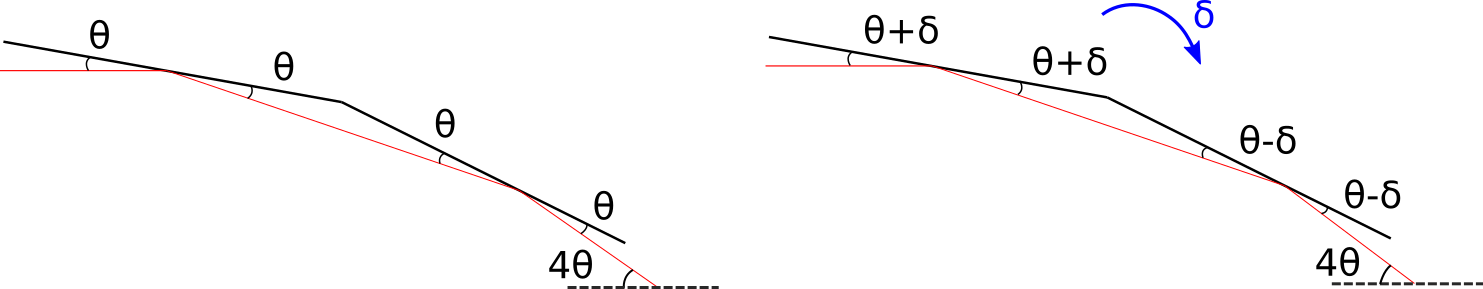
\includegraphics[width=10cm]{wolter_robustness.png}
\caption{2回反射による設置角度誤差のキャンセル}
\label{fig:wolter_robustness}
\end{figure}

このことは、2回反射が設置角度誤差に対して安定した結像性能を持つことの大きな理由である。
このような2回反射を利用した回転体ミラーをWolterミラーという。
Wolterミラーは近似的にアッベの正弦条件を満たし、無限遠方でのより広い領域を鮮明に結像することができる。\cite{VanSpeybroeck1972}

Wolterミラーの形状は、放物線、双曲線、楕円の3種類の2次曲線を組み合わせた図形の回転体として与えられる。
焦点を共有するように2つの2次曲線を配置することで、平行光を1点に集光する系を構成することができる。
WolterミラーにはI型(図\ref{fig:wolter_type_1})、II型(図\ref{fig:wolter_type_2})、III型(図\ref{fig:wolter_type_3})の3種類が存在し、I型は放物面内面・双曲面内面、II型は放物面内面・双曲面外面、III型は放物面外面・楕円面内面でそれぞれ2回反射する。
I型は応用性が高く、最も利用されているのWolterミラーとなる。
これは、2回とも内面で反射する構成であるため\ref{chap1_mirror_mandrel}節に述べるような凸形状から転写を行うマンドレル電鋳法が有効であることや、\ref{chap1_nested_wolter_mirror}節で述べるような複数枚のWolterミラーによるネスト構造を形成できる唯一の構成であることによる。
III型では2枚が覆いかぶさるように重ねた配置にすることができ、焦点距離を短くし光学系全体を小型化することができるが、I型に比べ加工・設置とも格段に難しくなるため、実用には至っていない。

\begin{figure}[b]
\centering
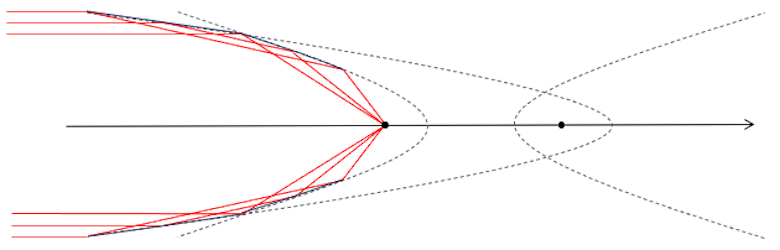
\includegraphics[width=10cm]{wolter_type_1.png}
\caption{Wolter I型}
\label{fig:wolter_type_1}
\end{figure}

\begin{figure}[b]
\centering
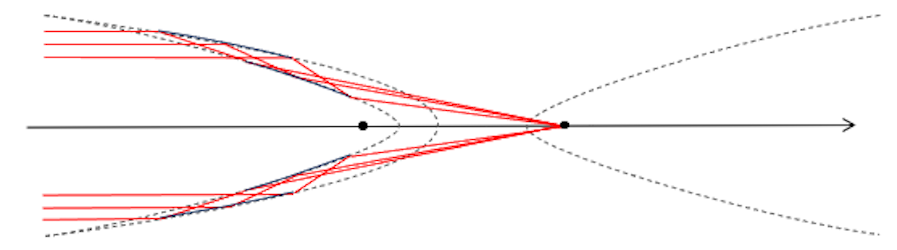
\includegraphics[width=10cm]{wolter_type_2.png}
\caption{Wolter II型}
\label{fig:wolter_type_2}
\end{figure}

\begin{figure}[b]
\centering
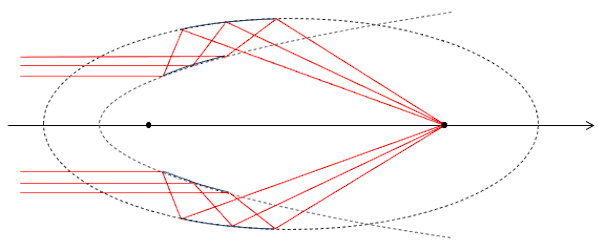
\includegraphics[width=10cm]{wolter_type_3.png}
\caption{Wolter III型}
\label{fig:wolter_type_3}
\end{figure}

\subsection{ネスト型Wolterミラー}
\label{chap1_nested_wolter_mirror}

Wolterミラーのような円筒形のミラー、特にX線を反射するため斜入射角が小さく設計されたミラーは、中空になっている内側部分を通過する光を集めることができず、集光強度を高める上で不都合である。
これを解決する方法として、図\ref{fig:nested_wolter_mirror}のように口径の異なるWolterミラーを内側に挿入するネスト構造がある。\cite{BuitragoCasas2017}

\begin{figure}[b]
\centering
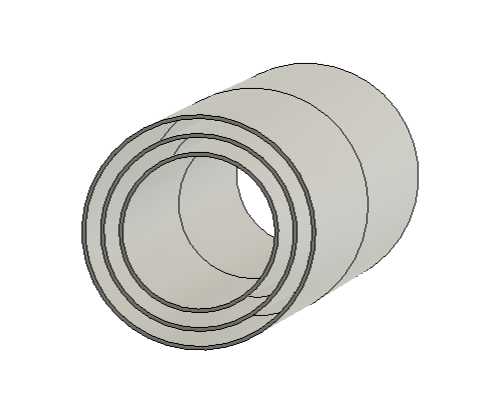
\includegraphics[width=8cm]{nested_wolter_mirror.png}
\caption{Nested Wolterミラーの例}
\label{fig:nested_wolter_mirror}
\end{figure}

ネスト構造にすることで受光面積を大きくすることができ、集光強度を上げることができる。
Wolterミラーでネスト構造を取ることができるのはI型のみであり、X線用結像光学系としてI型が最も有用である1つの理由となっている。
受光面積の観点で非常に有利であるNested Wolterミラーだが、ネストする枚数を増やすほどその設置が困難になるという問題がある。
ミラー同士の角度・光軸のずれなど、調整しなければならない誤差要因が増えるためである。
そのため、ネスト構造の構成後に光学系を統合的に計測する方法が必要になる。
また、ミラー同士をネストさせたあとにプローブを挿入して計測することは困難であるため、その統合的な評価は間接測定によって行われなければならない。

\clearpage
% -------------------------------------------------- %
% section
% -------------------------------------------------- %
\newpage

\section{FOXSI4におけるWolterミラー}
\label{chap1_background}

\subsection{FOXSI}
\label{chap1_foxsi}

2018年に打ち上げられたFOXSI3では太陽コロナのX線写真を撮影することに成功した。\cite{weko_20796_1}
図\ref{fig:foxsi-fullsun-image}はその撮影像の1枚である。
1 秒間に 250 枚のデータを約 6 分間取得し、活動領域のX線光子数の時間変化やX線のスペクトルが算出された。
FOXSI3に続いて2023年頃に打ち上げが予定されているFOXSI4では、太陽の状態を監視しフレアの発生が検知された時点でロケットを打ち上げることで、フレアの中期から後期を観測することを目指している。
既にフレア観測を行っているRHESSI\cite{Liu_2004}においては、撮影像の感度やダイナミックレンジが不十分であったため、Wolterミラーを用いた結像系により4 ~ 20 keV領域のX線をより鮮明に撮影することが目的となっている。\cite{2019AGUFMSH31C3315V}
JAXAの進めるミッションLynxでは、HPD 0.5 秒角の望遠鏡の搭載を大きな目標として掲げており\cite{Gaskin2019}、
FOXSI4に搭載予定のWolterミラーについてはそれに先立ってHPD 1 秒角の達成が目指されている。

\begin{figure}[h]
\centering
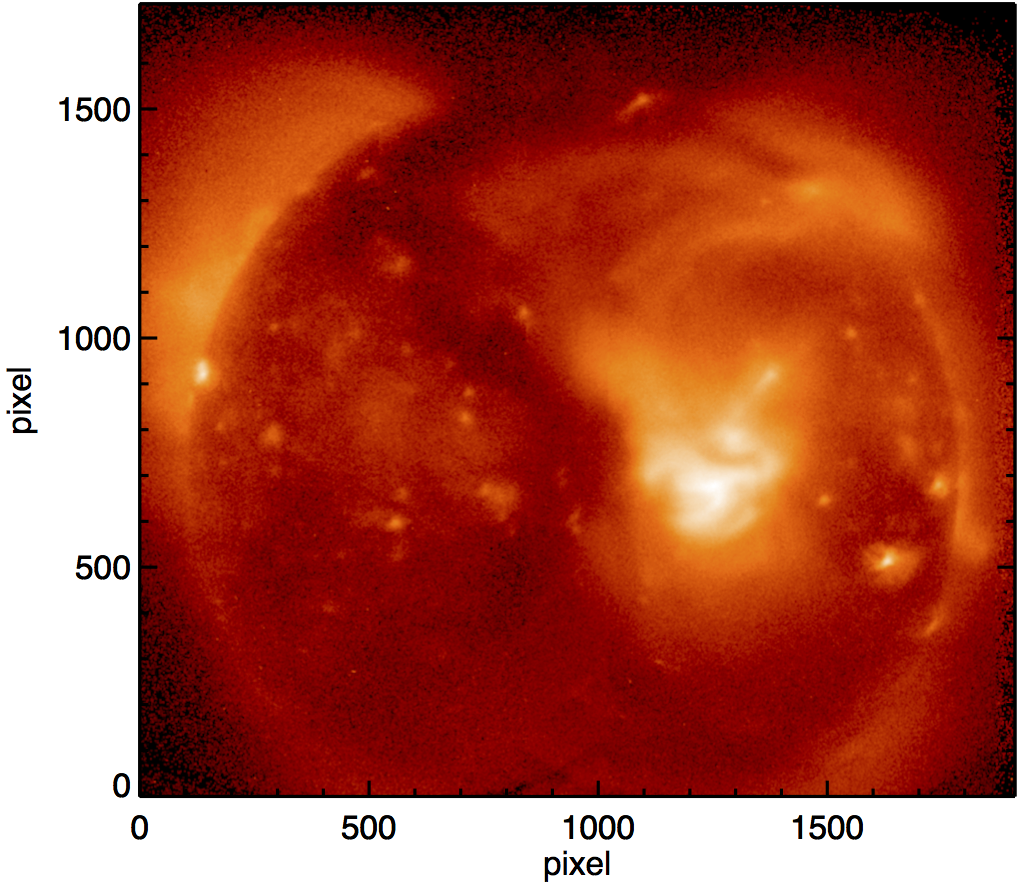
\includegraphics[width=6cm]{foxsi3-full-sun.png}
\caption{FOXSI-3 phoenix full sun soft X-ray image \cite{weko_20796_1}}
\label{fig:foxsi-fullsun-image}
\end{figure}

\subsection{Wolterミラーの設計}
\label{chap1_wolter_arrangement}
FOXSI4に搭載予定のX線用Wolterミラーは、放物面、双曲面の順に反射するI型に分類される。

以下では、開発対象となっているWolter I型のミラーの設計パラメータを図\ref{fig:wolter_params}に対応して表\ref{tb:wolter_params}に示す。

\begin{figure}[h!]
\centering
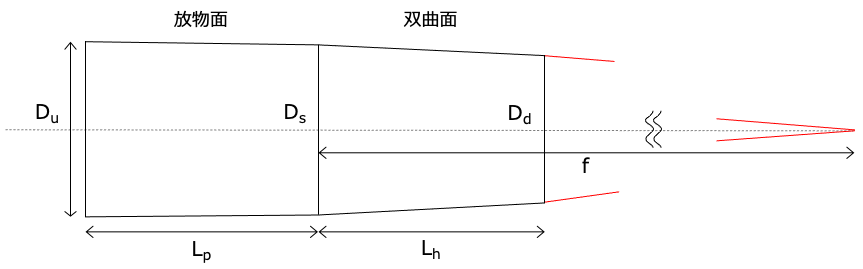
\includegraphics[width=12cm]{wolter_mirror_params.png}
\caption{Wolterミラーの設計変数}
\label{fig:wolter_params}
\end{figure}

\begin{table}[ht]
\begin{center}
  \begin{tabular}{|c|c|l|} \hline
    変数 & 値 & 説明 \\ \hline
    $d_u$ & 60.801 mm & 上流端開口直径 \\
    $d_s$ & 60.000 mm & 接合部直径 \\
    $d_d$ & 57.689 mm & 下流端開口直径 \\
    $l_p$ & 102.501 mm & 放物面部長さ \\
    $l_h$ & 97.499 mm & 双曲面部長さ \\
    $ml$ & 200.000 mm & ミラー全長 \\
    $f$ & 2000.000 mm & 焦点距離 \\ \hline
  \end{tabular}
  \caption{Wolterミラー各設計変数の値}
  \label{tb:wolter_params}
\end{center}
\end{table}

これらを図\ref{fig:wolter_profile}のように放物面部および双曲面部の設計半径として表すと、下式(パラメータは図\ref{tb:wolter_profile_constants})のようになる。
$f1$は座標系の平行移動に関して任意であるため、変数として表記する。

\begin{equation}
    r_p(z) = \sqrt{ -4p(z - p - f_2) } \\
\end{equation}

\begin{equation}
    r_h(z) = b \sqrt{ \frac{(z - (f_1 + f2) / 2)^2}{a^2} - 1.0 }
\end{equation}

\begin{figure}[h]
\centering
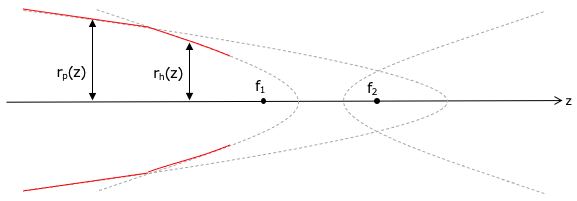
\includegraphics[width=10cm]{mirror_profile.png}
\caption{Wolterミラーの設計半径}
\label{fig:wolter_profile}
\end{figure}

\begin{table}[htb]
    \begin{center}
      \begin{tabular}{|c|c|l|} \hline
        定数 & 値 & 説明 \\ \hline
        $p$ & 0.0562 mm & 下流端開口直径 \\
        $a$ & 1000.056 mm & 放物面部長さ \\
        $b$ & 10.606 mm & 双曲面部長さ \\ 
        $f_1$ & 任意 & 焦点座標 \\
        $f_2$ & $f_1 + 2 \sqrt{ a^2 + b^2 }$  & 共焦点座標 (双曲線のもう一方の焦点) \\\hline
      \end{tabular}
      \caption{Wolterミラーの設計半径における定数}
      \label{tb:wolter_profile_constants}
    \end{center}
\end{table}


\subsection{マンドレル電鋳法}
\label{chap1_mirror_mandrel}

ここで、測定対象となるWolterミラーの製造プロセスについて述べる。
凹状になっている回転体形状のミラー内面を高精度に加工することは難しく、凸形状のマンドレルを高精度に加工し、これに対してさらに転写加工を行うという手法が提案されている。\cite{Mimura2018}
図\ref{fig:mandrel_plating_pictures}に回転楕円ミラーに対するマンドレル電鋳法の一連の流れを示す。

\begin{figure}[!ht]
\centering
\subfloat[高精度に加工されたマンドレル]{
    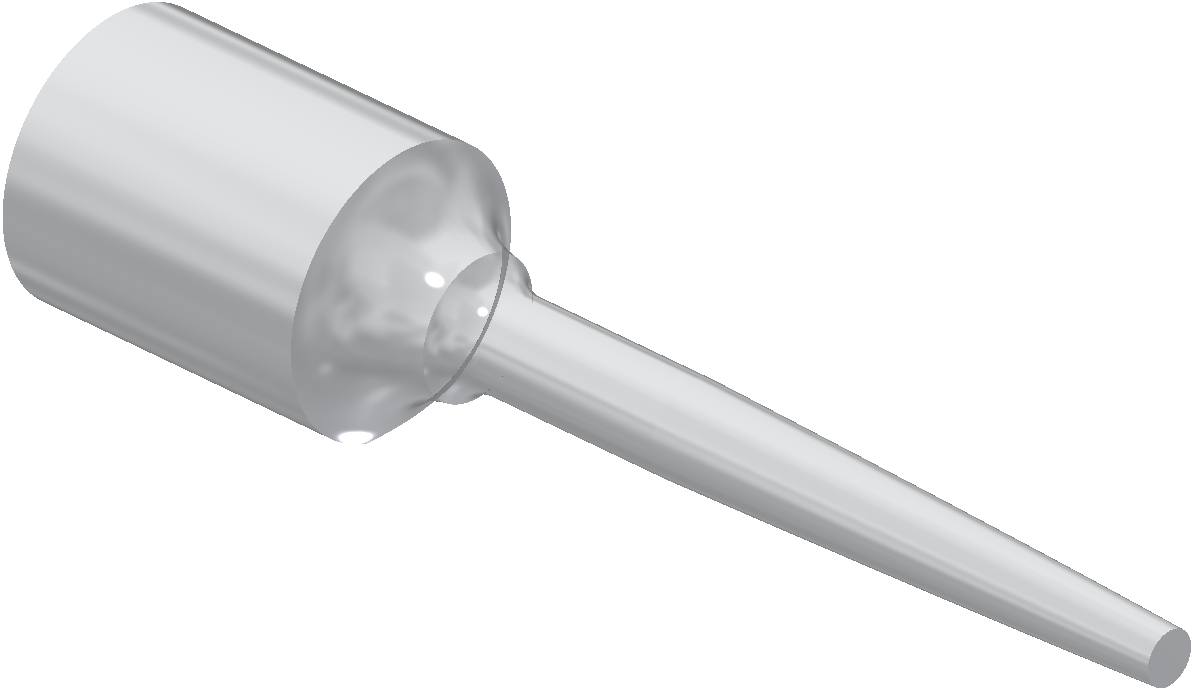
\includegraphics[width=4cm]{mandrel_before_plating.png}
    \label{fig:mandrel_before_plating}
}
\subfloat[マンドレルに転写されたミラー]{
    \centering
    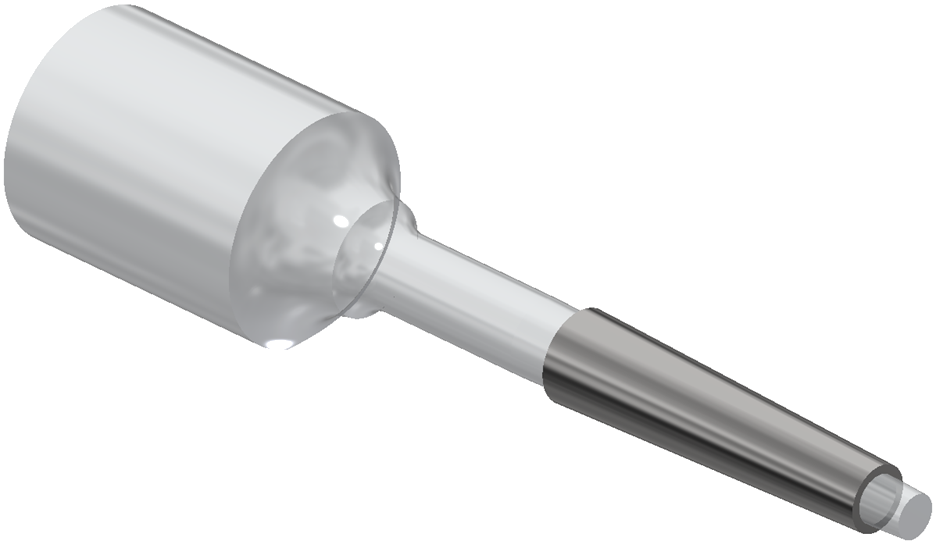
\includegraphics[width=4cm]{mandrel_after_plating.png}
    \label{fig:mandrel_after_plating}
}
\subfloat[取り外されたミラー]{
    \centering
    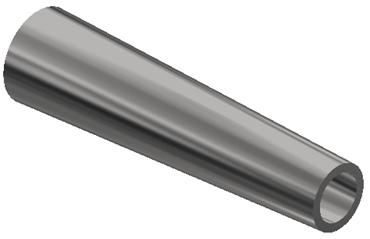
\includegraphics[width=4cm]{detached_mirror.png}
    \label{fig:detached_mirror}
}
\caption[]{マンドレル電鋳法の模式図}
\label{fig:mandrel_plating_pictures}
\end{figure}

3種類のWolterミラーのうち、2回の反射が内面において起こるI型では、同様の手法で加工が可能であり、既にこの方法で真円度誤差\SI{20}{\micro \metre}程度以下の精度でWolterミラーが作製されている。\cite{Yamaguchi2020}

\subsection{直接計測法}
\label{chap1_direct_measurement}

久米らは、図\ref{fig:profile_measurement_schematic}および図\ref{fig:profile_measurement}に示すように、中空形状のミラー内面に対して接触式変位計を用いて周方向形状誤差プロファイルおよび長手方向形状誤差プロファイルを数本ずつ取得し、さらにこれらを組み合わせることで3次元形状を決定するという方法を提案した。\cite{Kume2017}
しかし、これらの誤差プロファイル計測手法ではある始点からの変位量しか測定できず、直径や長手プロファイルの傾き(テーパー角)の情報を取得することができない。
また、長手方向の計測において始点の位置出しを行うことは非常に困難であり、中心軸の湾曲などの長周期形状誤差を測定することができない。
ミラーの結像性能を悪化させる要因を特定し作製過程へのフィードバックを行うためには、このような誤差プロファイル計測では得られない情報を補完する計測方法が必要である。
また、高精度に加工されたミラー内面に対して接触式のプロファイル計測を行うことは表面形状を悪化させる恐れがあるため好ましくなく、非接触式の計測方法の開発が求められている。

\begin{figure}[h]
\centering
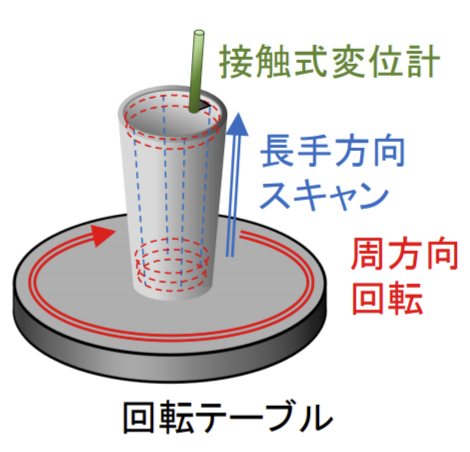
\includegraphics[width=5cm]{profile_measurement_schematic.png}
\caption{接触式誤差プロファイル計測}
\label{fig:profile_measurement_schematic}
\end{figure}

\begin{figure}[!ht]
\centering
\subfloat[長手方向形状誤差プロファイル]{
    \centering
    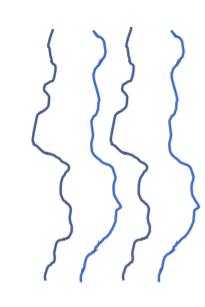
\includegraphics[height=4cm]{meridional_profile.png}
    \label{fig:meridional_profile}
}
\subfloat[周方向形状誤差プロファイル]{
    \centering
    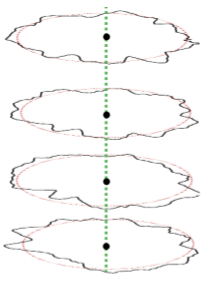
\includegraphics[height=4cm]{sagital_profile.png}
    \label{fig:sagital_profile}
}
\subfloat[3次元形状誤差プロファイル]{
    \centering
    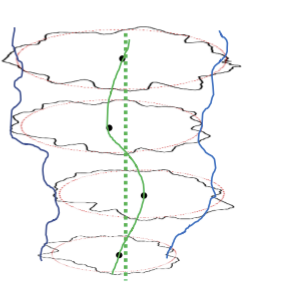
\includegraphics[height=4cm]{combined_profile.png}
    \label{fig:combined_profile}
}
\caption[]{プロファイル計測による3次元プロファイルの構成}
\label{fig:profile_measurement}
\end{figure}


\clearpage
% -------------------------------------------------- %
% section
% -------------------------------------------------- %
\newpage
\section{波面計測法によるミラー形状の解析}
\label{chap1_wave_metrics}

プロファイル計測では得られない情報を取得すること、またネスト構造のミラーを計測可能な間接測定であることという2つの要請を満足させる方法として、波動光学の理論を応用した波面計測法がある。
波動光学では、光波を複素スカラー場$U(P)=A(P)\exp(i\Phi(P))$として表現し、等位相面$\Phi(P)=const$を波面とよぶ。
一般に、ある光が1点に収束するとき、その光は収束点を中心とする球面状の波面を持つ。
結像用ミラーによって反射された光の波面は反射面の加工状の誤差や設置時の誤差を反映して変形し、その分布と変形量に対応して結像性能が悪化する。
波面計測法では、この波面のずれを波面誤差$\Delta\Phi(P)/k$として求め、結像性能を悪化させる要因を特定しその具体的な量を推定する。

\subsection{測定対象となるWolterミラーの特性}
\label{chap1_wolter_specific_feature}

口径が大きく射入射角の小さいWolterミラーはNAがやや低く、計測するべき波面は図\ref{fig:wolter_thinring}に示すように非常に細い輪帯状になる。
輪帯の幅(外円と内円の半径の差)は設計形状に対して\SI{363.3}{\micro \metre}であり、波面計測に求められる空間分解能は非常に高いものとなる。
波面精度を十分に確保しつつ、空間分解能が十分に高い波面計測法を開発する必要がある。

\begin{figure}[h!]
\centering
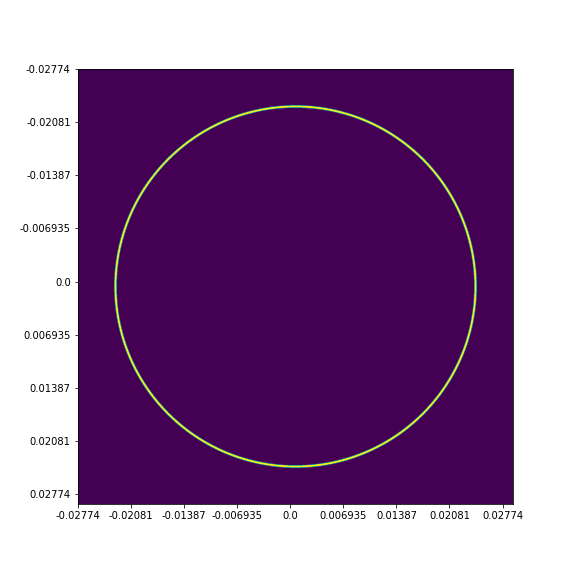
\includegraphics[width=7cm]{wolter_thinring.png}
\caption{Wolterミラー下流端面における集光波面}
\label{fig:wolter_thinring}
\end{figure}

\subsection{可視光による測定}
\label{chap1_visible_light_measurement}

高い空間分解能での測定という要求に加えて、測定装置が実験室内で実現・構成できるようなものであることが望まれる。
波面計測の光源としてX線を利用すれば、より微細な誤差情報を得ることができる。
しかし、波面計測に必要なコヒーレンス性の高いX線はその発生装置が非常に大掛かりなものであり、利用可能な施設は限られるため頻繁に測定実験を行うことは難しい。
FOXSIプロジェクトのような非常に短い期間での性能改善が求められる開発において、計測結果から加工プロセスへのフィードバックはより短いスパンでなされることが期待される。
そのため、本研究では入手性がよく研究や産業用途で広く利用されるHe-Neレーザ(波長 632.8 nm)を光源として用い、よりシンプルな光学配置による計測実験系を構築する。

\subsection{従来的な波面計測法}
\label{chap1_conventional_wave_metrics}
可視光領域での波面の計測手法として広く利用されているのが、シャックハルトマンセンサーである。
シャックハルトマンセンサは図\ref{fig:shack_hartmann_schematic}測定する光を2次元のレンズアレイに入射させ、集光点の位置ずれをカメラで検出することによって波面誤差を計測する。
理想的な球面波による校正を行ったとしても波面の安定性が高いとは言えず、X線用のミラーの形状精度に対して適用する上では大きな問題となる。
また、レンズアレイの大きさが空間分解能を決定するため、Wolterミラーの非常に細い輪体の計測には適さない。

\begin{figure}[h]
\centering
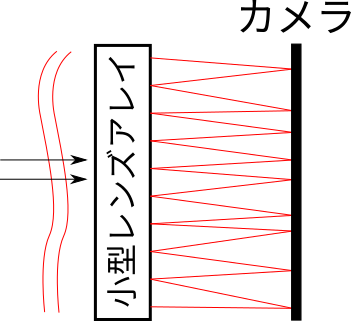
\includegraphics[width=5cm]{shack_hartmann_schematic.png}
\caption{シャックハルトマン干渉計}
\label{fig:shack_hartmann_schematic}
\end{figure}

\subsection{位相回復法}
シャックハルトマンセンサでは、実現するべき空間分解能に対して、素子のサイズが律速となってしまうという問題があった。
これに対して、位相回復法では空間分解能を測定領域の大きさという別の問題に置き換えることができる。
位相回復法とは、測定対象のミラーによって集光されたビームに位相物体を差し入れ、背後に現れる回折像の強度分布計測値から繰り返し計算によって位相情報を算出する方法である。
この手法の背景には、集光ビームの波動場の伝播がフーリエ変換の関係で与えられるという物理的法則がある。
伝播先の光波動場は元の波動場の空間周波数領域での表現になっており、これを広範囲に渡って測定することはもとの波面の小さな周期の情報を得ることに対応する。
素子の最小サイズによる律速がないため、測定する際の配置を工夫することで非常に高い空間分解能が実現できる。
本研究では、位相回復法を計測法として採用し、より高い空間分解能が実現される形状測定装置の構成について検討する。

\clearpage
% -------------------------------------------------- %
% section
% -------------------------------------------------- %
\newpage

\section{本論文の目的および構成}
\label{chap1_purpose}

ここまで、X線天文学における結像用Wolterミラーの有用性、およびFOXSI4に搭載されるWolterミラーの非接触式で簡易的な測定装置の開発の必要性について説明した。
本研究では、\ref{chap1_wave_metrics}節で述べたように可視光光源を用いた位相回復法による計測装置の提案および検証実験を行う。
まず、\ref{chap3}章で様々な位相回復法について検討し、計測に用いる手法を提案した上で、シミュレーションにより手法の正当性を検証する。
\ref{chap5}章では、実際に加工されたFOXSI4用のWolterミラーに対して計測実験を行い、その結果について考察する。
最後に、\ref{chap6}章で考察、結論および今後の展望について述べる。

%%%%%%%%%%%%%%%%%%%%%%%%%%%%%%%%%%%%%%%%%%%%%%%%%%%%%%%%%%%%%%%%%%%%%%%%%%%%%
%%% Local Variables:
%%% mode: katex
%%% TeX-master: "../thesis"
%%% End:

\chapter{Wolterミラーの誤差応答シミュレーション}
\thispagestyle{empty}
\label{chap2}
\graphicspath{{chap2/figure/}}
\minitoc

\newpage
%%%%%%%%%%%%%%%%%%%%%%%%%%%%%%%%%%%%%%%%%%%%%%%%%%%%%%%%%%%%%%%%%%%%%%%%%%%%%


% ================================================== %
% section
% ================================================== %
\section{諸言}
\label{chap2_introduction}

Wolterミラーを光学系に組み込んで利用する際、大きく分けて2つの誤差によってその理想の集光・結像が損なわれる。
ひとつは設計曲面と実際に加工されたミラー表面の形状の誤差、もうひとつはミラー設置時の位置・姿勢の誤差である。

これらを与えたとき集光点の様子がどのようになるか、また集光点の変化として許容できる誤差の範囲はどれほどなのかを見積もることは、Wolterミラー評価の重要な軸となる。
6章では、加工されたミラーに対して測定実験を行い、本章で計算した許容誤差との比較・検討を行う。
なお、以下では光軸上を川になぞらえて光源の側を上流側、集光点の側を下流側と呼ぶことにする。

\clearpage
% ================================================== %
% section
% ================================================== %
\newpage
\section{誤差の評価と許容される誤差}
\label{chap2_beam_evaluation_standard}

結像または集光を行う光学系の是非が、集光面での波面が理想からどれだけ離れているかということで評価されるということを先に述べた。
いま、理想の集光波面との差異を定量的に評価するためには、具体的な評価軸が必要である。
そこで主に用いられるのが、Strehl比、HPD、FWHMの3つの特徴量である。

\subsection{Strehl比}
\label{chap2_strehl_ratio}
主に集光光学系の文脈において、理想の集光状態を「回折限界集光」と呼ぶ。
回折限界集光の状態にあるかどうかを判別する1つの指標として用いられるのが、Strehl比である。
Strehl比とは、実際の集光波面における最大値と回折限界時の集光波面における最大値の比として定義される。
つまり、振幅を$I(\mathbf{r})$として

\[
r_{\mathrm{Strehl}} = \frac{ \max{\sqrt{I(\mathbf{r})} } }{ \max{ \sqrt{I_{\mathrm{ideal}}( \mathbf{r} )} } }
\]

と定まる。
図\ref{fig:strehl_explanation}にその模式的なグラフを示す。
Strehl比を評価する基準として、Marechal基準\cite{BornWolf:1999:Book}が知られている。
Marechal基準では、Strehl比が0.8以上であるときその系は回折限界集光をしている、とする。
この0.8という値には体系的な根拠はなく、解析・実験における経験的な指標として扱われている。
本論文では、この慣例を踏襲し、0.8を閾値としてStrehl比を評価する。

\begin{figure}[h]
\centering
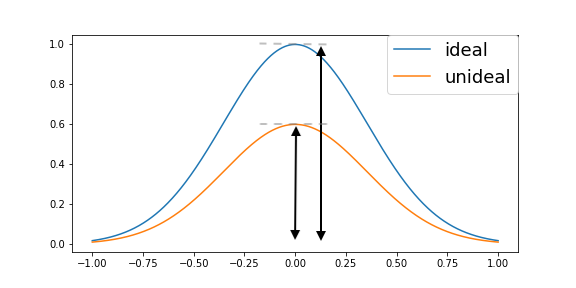
\includegraphics[width=10cm]{strehl.png}
\caption{Strehl比計算の模式図}
\label{fig:strehl_explanation}
\end{figure}

\subsection{HPD (Half Power Diameter)}
\label{chap2_hpd}

Strehl比による比較検討では「回折限界集光をしているか」に主眼を置いているが、天文用Wolterミラーのように達成すべき角度分解能が決まっている場合では、直接その分解能要求を満たしているかどうかを判定するのが実用的である。
分解能を決定するのは、焦点面におけるビームの集光サイズであり、これは大きく2つの定義によって議論される。
その一つが、Half Power Diameter(HPD)である。HPDの定義は「焦点面上の全強度の50\%の強度を含む円の直径」である。つまり、
\[
    \sum_{d\leq d_{\mathrm{HPD}}} \sqrt{ I(\mathbf{r}) } = \frac{1}{2} \sum \sqrt{ I(\mathbf{r}) }
\]
を満たすような直径$d_{\mathrm{HPD}}$として定義される。
図\ref{fig:hpd_explanation}にその例を示す。
この赤円の内側の強度総和値は、全体の強度総和値の半分になっている。

\begin{figure}[!ht]
\centering
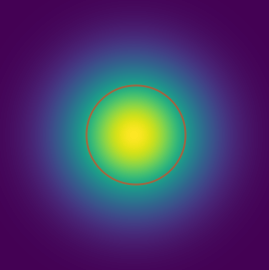
\includegraphics[width=6cm]{HPD.png}
\caption{HPDの例}
\label{fig:hpd_explanation}
\end{figure}

あるHPDを持つようなのふたつの結像点を分離できるような限界の配置が図\ref{fig:hpd_resolution_limit}のときであるとするならば、1秒角分解能という達成目標は図\ref{fig:hpd_arcsecond}が示すようなHPDで言い換えることができる。
つまり、ミラー上流端中心から半径を見込む角度がちょうど1秒角となるようなHPDが達成目標となる。
具体的には、ミラー上流端開口から焦点面までの距離が
HPDを指標とした評価では、これを基準とする。

\begin{figure}[ht]
\centering
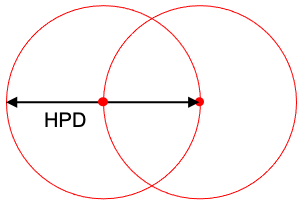
\includegraphics[width=6cm]{hpd_resolution_limit.png}
\caption{解像限界の図}
\label{fig:hpd_resolution_limit}
\end{figure}

\begin{figure}[ht]
\centering
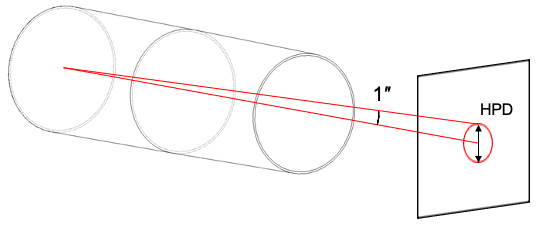
\includegraphics[width=12cm]{hpd_arcsecond.png}
\caption{HPDと結像分解能の関係}
\label{fig:hpd_arcsecond}
\end{figure}


\subsection{FWHM (Full Width Half Maximum)}
\label{chap2_fwhm}

HPDに並んでビーム集光サイズの評価として用いられるのが、FWHM(Full Width Half Maximum)である。
こちらは焦点面を集光点を通る直線によって切断したプロファイルに対して、「焦点面における最大値の半分の値を取る2点の距離」と定められる。
図\ref{fig:fwhm_explanation_profile}は1つのプロファイルに対するFWHMの例である。
切断する直線には任意性があるため、通常は図\ref{fig:fwhm_explanation}のように水平方向と鉛直方向の切断しこれを評価する。

\begin{figure}[ht]
\centering
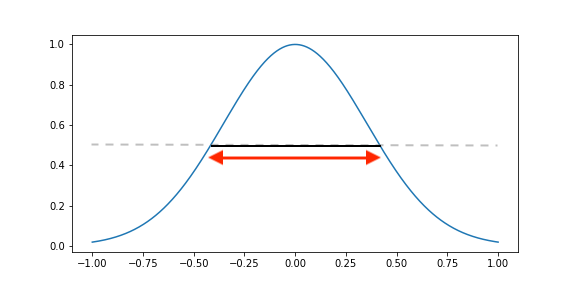
\includegraphics[width=10cm]{FWHM.png}
\caption{FWHMの例}
\label{fig:fwhm_explanation_profile}
\end{figure}

\begin{figure}[!ht]
\centering

\subfloat[horizontal]{
    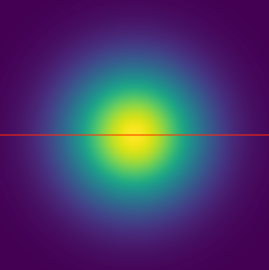
\includegraphics[width=6cm]{FWHM_horizontal.png}
    \label{fig:fwhm_explanation_horizontal}
}
\subfloat[vertical]{
    \centering
    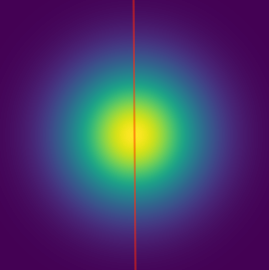
\includegraphics[width=6cm]{FWHM_vertical.png}
    \label{fig:fwhm_explanation_vertical}
}
\caption[]{切断の例 水平:\subref{fig:fwhm_explanation_horizontal}, 鉛直:\subref{fig:fwhm_explanation_vertical}}
\label{fig:fwhm_explanation}
\end{figure}


\clearpage
% ================================================== %
% section
% ================================================== %
\newpage

\section{Wolterミラーにおける光学波動場の伝播}
\label{chap2_wolter_diffraction_apporoximation}
本節では、本研究で測定対象とするWolterミラーの系において適用するべき波動場伝播の近似公式について説明する。
光学波動場の伝播に関しての詳細は付録において解説する。
まず、1章\ref{chap1_wolter_arrangement}節で示したパラメータについて、Fresnel回折近似が成り立つことを確認する。
Fresnel回折近似が成り立つための条件は、近似で切り捨てる微小項が1 radより十分小さいときであり、これは式\ref{eqn:fresnel_approximation_conditon}で表される。
ただし$z$は伝搬距離、$\lambda$は波長、$(x, y), (\xi, \eta)$は実空間および逆空間の座標を表す。

\begin{equation}
\label{eqn:fresnel_approximation_condition}
    \frac{\pi}{4\lambda} \max \left\{ (x-\xi)^2 + (y-\eta)^2 \right\}^2 / z^3 \ll 1
\end{equation}

パラメータを代入して確認すると、$\text{(左辺)=}$

\clearpage
% ================================================== %
% section
% ================================================== %
\newpage

\section{位相接続(位相アンラッピング)}
$\sin$関数などの周期関数は、逆関数の値域が周期以下の大きさしか持たないため、完全にもとの入力を戻すことはできない。
複素波動場の位相分布についても同様である。
$\exp(i\phi)$は周期$2\pi$の関数であり、逆関数は$\arg\{\exp(i\phi)\}=\phi \mod{2\pi}$と位相の$\mod{2\pi}$での剰余を返す。
故に、位相分布が本来なめらかな関数として与えられたとしても、それが$2\pi$を超えるような範囲に渡って分布する際には必ずどこかで不連続に位相が飛んでしまう。
例えば、$y = f(x) = 4 x + \sin(x) - 2 \sin(2 x) - 4 \sin(10 x) \quad (x \in [0, 1])$に対して$z = \arg\{\exp(iy)\}$を取ると、図\ref{fig:wrapped_graph_example}のようになる。

\begin{figure}[ht]
\centering
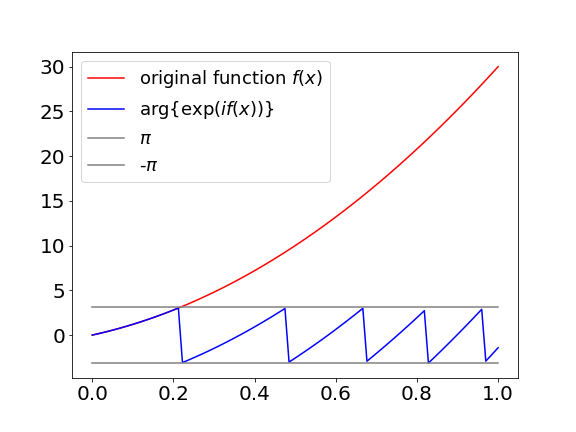
\includegraphics[width=10cm]{before_unwrap.png}
\caption{arg関数によって不連続になったグラフの例}
\label{fig:wrapped_graph_example}
\end{figure}

これに対して、離散化された領域において1ピクセルで$2\pi$以上のジャンプはないものと仮定して順番に接続を行うことで、なめらかな位相分布を取り戻すことができる。
これを位相接続あるいは位相アンラップといい、1次元の場合の最もシンプルなアルゴリズムは離散列$y[n] = f(x[n])$および$z[n]=\arg\{\exp(iy[n])\}$に対してAlgorithm \ref{alg:unwrap_1d}のようになる。

\begin{algorithm}                      
\caption{1次元アンラップの例}         
\label{alg:unwrap_1d}                          
\begin{algorithmic}
    \FOR{n = 1 \ldots N-1}
        \STATE $z[n] \leftarrow z[i] + \begin{cases}
           -2 \pi & (z[n] + \pi < z[n]) \\
           0 & (z[n] - \pi \leq z[n] \leq z[n] + \pi) \\
           2 \pi & (z[n] < z[n] - \pi)
        \end{cases}$
    \ENDFOR
\end{algorithmic}
\end{algorithm}

2次元のリング状の領域に対しても同様に行うことができ、接続するべき2次元位相分布内においてピクセルの走査順序を決めれば、1次元の場合と同じアルゴリズムで接続を行うことができる。
ミラー波面計測においては、経験的に十分な空間分解能があれば$2\pi$以上のジャンプはないと考えてよいとされており、本研究でも同様にその仮定をおいて測定を行う。

\clearpage
% ================================================== %
% section
% ================================================== %
\newpage



\section{シミュレーションの方法}
この節では、シミュレーションの方法について述べる。


\clearpage
% ================================================== %
% section
% ================================================== %
\newpage

\section{計算条件}
6章で実際に利用する測定対象のミラーについて、誤差応答のシミュレーションを行う。

図\ref{corona_spectrum}は、FOXSI3において撮影されたデータから解析された太陽コロナの活動領域におけるX線スペクトルである。\cite{2019AGUFMSH31C3315V}
これをもとに考えれば、測定対象となるX線のエネルギーは数百eVから4keV程度であることになる。

\begin{figure}[ht]
\centering
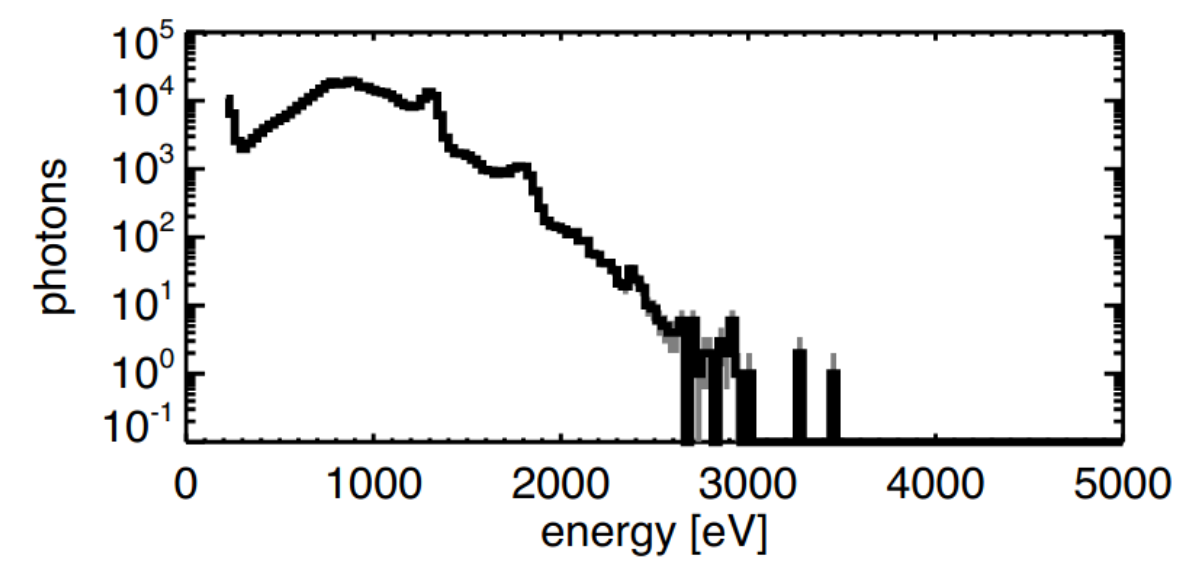
\includegraphics[width=6cm]{corona_spectrum.png}
\caption{太陽コロナ活動領域のX線スペクトル}
\label{fig:corona_spectrum}
\end{figure}

本章では表\ref{tb:simulation_target_energy}に示すように、太陽コロナの観測の際に測定対象となるX線領域のうち数点、および5章の波面計測実験に用いる可視光ビームの波長を対象にシミュレーションを行う。

\begin{table}[!ht]
\begin{center}
  \begin{tabular}{|c|c|} \hline
    エネルギー & 波長 \\ \hline
    19.59 eV & 632.8 nm \\
    300.0 eV & 4.133 nm  \\
    1.0 keV & 1.240 nm  \\
    3.0 keV & 0.413 nm  \\ \hline
  \end{tabular}
  \caption{シミュレーションで入力する波長・エネルギー}
  \label{tb:simulation_target_energy}
\end{center}
\end{table}

\clearpage
% ================================================== %
% section
% ================================================== %
\newpage

\section{理想集光}

まず、誤差入力を与える前に、誤差のない理想的なミラー形状に対する集光面強度分布を計算し、その特徴について述べる。

\begin{comment}
\begin{figure}[!ht]
\centering

\subfloat[可視光(632.8nm)]{
    \includegraphics[width=3cm]{ideal/visible_light_focus_abs.png}
    \label{fig:visible_light_ideal_focus_abs}
}
\subfloat[300eV]{
    \centering
    \includegraphics[width=3cm]{ideal/300eV_focus_abs.png}
    \label{fig:300eV_ideal_focus_abs}
}
\subfloat[1keV]{
    \centering
    \includegraphics[width=3cm]{ideal/1keV_focus_abs.png}
    \label{fig:1keV_ideal_focus_abs}
}
\subfloat[3keV]{
    \centering
    \includegraphics[width=3cm]{ideal/3keV_focus_abs.png}
    \label{fig:3keV_ideal_focus_abs}
}
\caption[]{理想的なミラーの各波長に対する集光波面}
\label{fig:fwhm_explanation}
\end{figure}
\end{comment}

表\ref{tb:ideal_focus_evaluation}にそれぞれの波長に対するHPDおよびFWHMを示す。
理想集光の場合は集光波面が回転対象になっているため、FWHMは任意の横方向の1本のプロファイルに対してのみ示す。

\begin{table}[!ht]
\begin{center}
  \begin{tabular}{|c|c|c|c|c|} \hline
    項目 & 可視光(632.8nm) & 300eV & 1keV & 3keV \\ \hline
    HPD & 8.989 mm & \SI{23.38}{\micro \metre} & \SI{20.37}{\micro \metre} & \SI{19.45}{\micro \metre} \\
    FWHM & \SI{19.53}{\micro \metre} & \SI{0}{\micro \metre} & \SI{0}{\micro \metre} & \SI{0}{\micro \metre} \\ \hline
  \end{tabular}
  \caption{理想集光の場合のHPDおよびFWHM}
  \label{tb:ideal_focus_evaluation}
\end{center}
\end{table}

\clearpage
% ================================================== %
% section
% ================================================== %
\newpage

\section{各誤差入力に対するシミュレーション}
\label{chap2_simulation_error_response}

本節では、ミラーの製造過程で発生する様々な誤差要因についてその概要を示した上で、それを与えた時の集光波面の変化についてシミュレーションを行う。
シミュレーションでは、\ref{chap2_beam_evaluation_standard}節で述べた3つの評価基準に対応した、許容誤差の閾値を示す。
まず、Strehl比の解析により回折限界集光を達成する上で許容される誤差を評価し、続いて天文用Wolterミラーの達成目標として定めた1秒角分解能の達成に対して求められる許容誤差をHPDおよびFWHMを用いてレイリーの解像限界に照らし合わせて評価する。

\subsection{直径誤差}

\subsection{扁平誤差}

\subsection{周方向形状誤差}

\subsection{長手方向形状誤差}

\subsection{設置角度誤差}

\subsection{設置位置誤差}


\clearpage
% ================================================== %
% section
% ================================================== %
\newpage


\clearpage
% ================================================== %
% section
% ================================================== %
\newpage
\section{収差解析}
\label{chap2_simulation_zernike_analysis}

\ref{chap2_simulation_error_response}節では、ミラー加工において生じる様々な誤差を紹介するとともに、その誤差入力についてのシミュレーションを行った。
本節では、\ref{chap3}章で述べる位相回復によって得られた波面情報から各誤差への分解を行うための解析方法について検討する。

\subsection{Zernike収差}

\subsection{輪帯状の位相分布に対するZernike収差}


\subsection{各誤差に起因する収差の解析}



\section{結論}
\label{chap2_conclusion}



%%%%%%%%%%%%%%%%%%%%%%%%%%%%%%%%%%%%%%%%%%%%%%%%%%%%%%%%%%%%%%%%%%%%%%%%%%%%%
%%% Local Variables:
%%% mode: katex
%%% TeX-master: "../thesis"
%%% End:

\chapter{Wolterミラー評価実験の手法に関する検討}
\thispagestyle{empty}
\label{chap3}
\graphicspath{{chap3/figure/}}
\minitoc

\newpage
%%%%%%%%%%%%%%%%%%%%%%%%%%%%%%%%%%%%%%%%%%%%%%%%%%%%%%%%%%%%%%%%%%%%%%%%%%%%%


% ================================================== %
% section
% ================================================== %
\section{諸言}
\label{chap3_introduction}

2章では、Wolterミラーの誤差応答シミュレーションを行い、各種形状誤差によって生じる波面誤差分布を計算した。
本研究の目的であるミラー上の形状誤差量の測定は、それぞれの誤差に対応する波面誤差分布を基底としてミラー下流端面における波面を分解することによってなされる。
本章では、波面計測に用いる位相回復法について基礎的な理論を述べた上で様々な手法について検討し、計測に用いる手法を決定、提案する。
また、提案された手法について測定対象の天文用Wolterミラーに合わせたシミュレーションを行い、その有効性を確認する。

\clearpage
% ================================================== %
% section
% ================================================== %
\newpage

\section{手法の決定に関する方針}
\label{chap3_method_choice_policy}

本節では、手法の検討に先立って、計測方法に対して要請される事項について述べる。

\subsection{高空間分解能}
\label{chap3_high_spatial_resolution}
1章で述べたように、測定対象となるWolterミラーで波面計測を行う際の大きな問題点は、2回反射されたビームが非常に細い輪帯形状をなすことである。
この極めて細い輪帯波面を測定し、形状誤差の情報を計算するためには、形状誤差が波面の動径方向に与える変化を十分な空間分解能で計算できなければならない。
当然、動径方向分解能が高くなるほど長手方向の形状誤差の位置分解能も上がるが、ここでは最低限の条件として3次のコマ収差を検出できること、すなわち動径方向に3画素の分解能を持つことを要請として定める。

\subsection{ダイナミックレンジ}
\label{chap3_dynamic_range}

位相回復計算を行う上で非常に重要な要素の1つが、カメラのダイナミックレンジである。
測定する強度分布において一定値を下回る点では強度が0として検出されてしまうため、同じ強度分布を持つ系であっても回復計算に対して有効な領域はダイナミックレンジによって左右される。
逆に、同じダイナミックレンジに対して有効な領域の大小によって回復計算の収束性や得られる情報の質が変化する。
本研究で用いるCCDカメラのパラメータは表\ref{tb:ccd_camera_params}の通りであり、これに対して回復計算が実行できるような手法であることが要請される。

\begin{table}[!ht]
\begin{center}
  \begin{tabular}{|c|c|l|} \hline
    項目 & 値 \\ \hline
    製品名 & Bitran BQ-85M \\
    ピクセルサイズ & 9.0 um \\
    画素 & 4096 $\times$ 4096 \\
    受光面積 & 36.9 mm $\times$ 36.9 mm \\
    A/Dコンバータ & 16bit (65535階調) \\ \hline
  \end{tabular}
  \caption{CCDカメラのパラメータ}
  \label{tb:ccd_camera_params}
\end{center}
\end{table}

\clearpage
\newpage

% ================================================== %
% section
% ================================================== %

\section{位相回復法}

\subsection{位相回復法の概要}
\label{chap3_phase_retrieval_introduction}

1章\ref{chap1_wave_metrics}でも述べた通り、位相回復法は波面計測法の一種であり、CCDなどの受光素子で計測された強度値の情報から位相分布を算出する方法である。
より具体的には、測定対象の波面の存在する領域について、$N \times N$の強度計測値を元に$N \times N$の位相を求める。
位相回復法には様々な手法が存在するが、いずれの方法においても基本的な方針は共通している。
未知数となっている位相をすべて決定するためには、それら未知数を含む十分な本数の方程式を立式する必要がある。一般に、求める光学波動場において強度と位相の間に拘束関係はない。
そこで、測定対象の波面領域に加えて光の進行方向にもう1つ未知の波面領域を定め、これら2つの領域間での光学波動場の伝播を関係式として与えることで、求める未知数を含む方程式を得ることができる。
これを図\ref{fig:phase_retrieval_policy}に示す。
波動場の伝播は$N \times N$の離散領域に対して$N \times N$本の数式で表される。
これだけでは未知数が$3N \times N$個に対して方程式が$N \times N$本と少なく、未知数を全て決定することができない。
そこで、未知数を減らす、もしくは成立する方程式を増やすといった工夫を行うことで、解を決定するという方針を取る。

\begin{figure}[!ht]
\centering
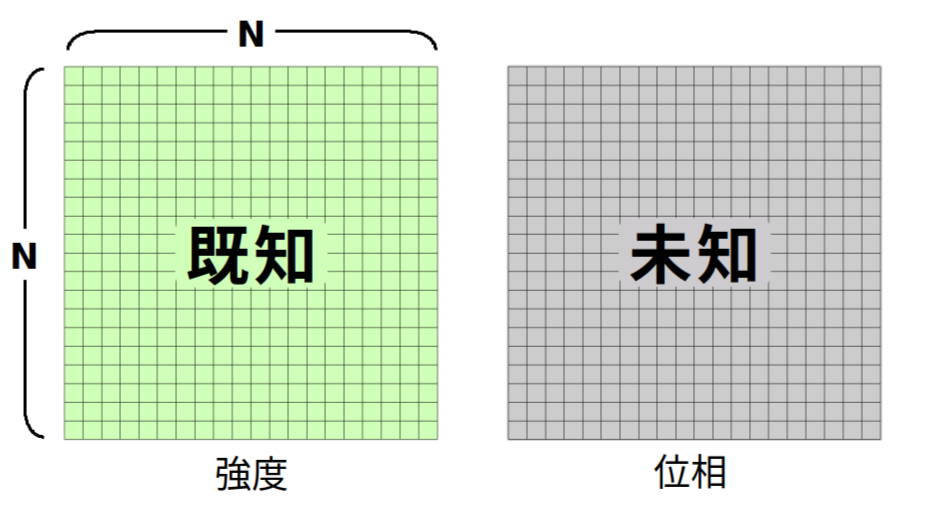
\includegraphics[width=6cm]{phase_retrieval_problem.png}
\caption{位相回復問題}
\label{fig:phase_retrieval_problem}
\end{figure}

\begin{figure}[!ht]
\centering
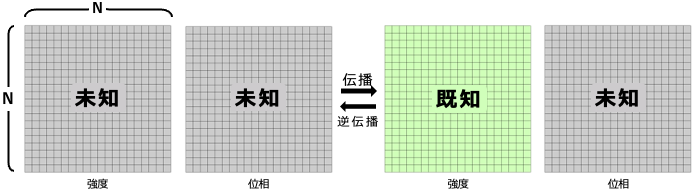
\includegraphics[width=12cm]{phase_retrieval_policy.png}
\caption{位相回復法の方針}
\label{fig:phase_retrieval_policy}
\end{figure}

\subsection{サンプリング定理}
\label{chap3_sampling_theorem}

ある2つの平面の間で光波の伝播が起こるとき、この2つの領域が遠方である場合あるいは光波が伝播先で収束するような場合には、その伝播はフーリエ変換の関係によって与えられる。(ref hoge)
つまり、二平面はそれぞれもう一方の周波数領域(波数領域)での表現になっており、カメラで取得される離散領域に対して適用し離散フーリエ変換を行うとき、サンプリング定理によって互いに領域サイズは拘束関係にある。
逆空間の領域はナイキスト周波数$k_s$に対して$[-k_s, k_s]^2$として与えられるので、これを実空間、逆空間の空間分解能に対して表すと、式\ref{eqn:sampling_theorem_px},\ref{eqn:sampling_theorem_size}のようになる。
ただし、波長を$\lambda$、焦点距離を$f$とし、領域の1画素の一辺を$\Delta L_r, \Delta L_f$、領域全体の一辺を$L_r=N \Delta L_r, L_f = N \Delta L_f$とする。

\begin{eqnarray}
  \Delta L_{\mathrm{real}} \Delta L_{\mathrm{reciprocal}} = \frac{f  \lambda}{N} \label{eqn:sampling_theorem_px} \\
  \Leftrightarrow 
  L_{\mathrm{real}} L_{\mathrm{reciprocal}} = N f \lambda \label{eqn:sampling_theorem_size}
\end{eqnarray}

これは、ミラー下流端面における空間分解能が高い波面領域を取ることは、焦点面において広い波面領域を取ることと等価である。

\clearpage
\newpage

\subsection{孤立条件の利用}
\label{chap3_solitude_introduction}
主にCDI(コヒーレント回折イメージング)の文脈において、波動場が到達しない領域を定数0として与えることで、未知数をの総数を激減させるという方法が多く取られる。
CDIとは、図\ref{fig:cdi_schematic}に示すように、サンプルに集光ビームを照射し、その回折像を見ることでそのサンプルの内部構造を解析する方法である。

\begin{figure}[!ht]
\centering
\includegraphics[width=12cm]{cdi_schematic.png}
\caption{コヒーレント回折イメージングの概要}
\label{fig:cdi_schematic}
\end{figure}

位相回復法によってディテクターでの位相およびサンプル面における位相・強度を求めることで、サンプル各点における透過率を求めることが目標となる。
このような系においては、カメラの画素をより細かく取ることにより、対応するサンプル面での領域がサンプルより大きく広がるため、この領域には波面が存在しないという仮定を用いて回復計算を行うことができる。
Wolterミラーの計測に用いる場合は、焦点面にCCDカメラを配置し、ミラーの輪帯に対して孤立条件を適用することになる。
この方針に則って、位相回復計算を行う最もシンプルなアルゴリズムがBIO(Basic Input-Output) Algorithmである。
疑似コードをAlgorithm\ref{alg:bio}に示す。

\newcommand{\pos} {
    \mathbf{r}
}
\newcommand{\rpos} {
    \mathbf{q}
}

\begin{algorithm}                      
\caption{BIO Algorithm}         
\label{alg:bio}                          
\begin{algorithmic}
    \STATE $\phi_0(\pos)$
      = $\begin{cases}
        \mathrm{rand} & (\pos \in S) \\
        0 & (\pos \notin S)
      \end{cases}$
    \FOR{n = 0 \ldots N-1}
    \STATE $\Psi_n(\rpos) = \mathcal F [\phi_n(\pos)]$
    \STATE $\Psi_{n+1}(\rpos) = \sqrt{I(\rpos)} \exp \left( i \arg \Psi_n(\rpos) \right)$ 
    \STATE $\phi_n'(\pos) = \mathcal F^{-1} [\Psi_{n+1}(\rpos)]$
    \STATE $\phi_{n+1}(\pos)
      = \begin{cases}
          \phi_n'(\pos) & (\pos \in S) \\
          0 & (\pos \notin S)
      \end{cases}$
    \ENDFOR
\end{algorithmic}
\end{algorithm}

これを改良し、サポートによる射影を弱めることで収束性を高めたのが、HIO(Hybrid Input-Output) Algorithmである。
疑似コードはAlgorithm\ref{alg:hio}のようになる。

\begin{algorithm}                      
\caption{HIO Algorithm}         
\label{alg:hio}                          
\begin{algorithmic}
    \STATE $\phi_0(\pos)$
      = $\begin{cases}
        \mathrm{rand}(0,1) & (\pos \in S) \\
        0 & (\pos \notin S)
      \end{cases}$
    \FOR{n = 0 \ldots N-1}
    \STATE $\Psi_n(\rpos) = \mathcal F [\phi_n(\pos)]$
    \STATE $\Psi_{n+1}(\rpos) = \sqrt{I(\rpos)} \exp \left( i \arg \Psi_n(\rpos) \right)$ 
    \STATE $\phi_n'(\pos) = \mathcal F^{-1} [\Psi_{n+1}(\rpos)]$
    \STATE $\phi_{n+1}(\pos)
      = \begin{cases}
          \phi_n'(\pos) & (\pos \in S) \\
          \phi_n(\pos) - \beta \phi_n'(\pos) & (\pos \notin S)
      \end{cases}$
    \ENDFOR
\end{algorithmic}
\end{algorithm}

位相回復計算が収束するかどうかを決める最大の要因の1つが、オーバーサンプリング比、つまり試料に対してどれだけ大きな領域を取って計算できるかということである。
これは、カメラの空間分解能によって決まる。
位相回復計算が収束するために必要な最低限の条件として、FFTで結ばれる関係式の数が未知数の数を上回らなければならない。
Friedel則による対称性などを考慮すると、取得する総ピクセル数が回復する試料のピクセル数の2倍になっていなければいけないことになる。\cite{Latychevskaia2018}
実際にはノイズが乗ったり、直接通過する光が入射しないようにビームストップを配置したりといった事情から、2倍より大きくなければならない。

ミラーに適用する際には、図\ref{fig:solitude_schematic}のように焦点面にCCDカメラを配置し、下流端面の輪帯が正方形状の領域に対して疎であることを利用して計算を行う。

\begin{figure}[!ht]
\centering
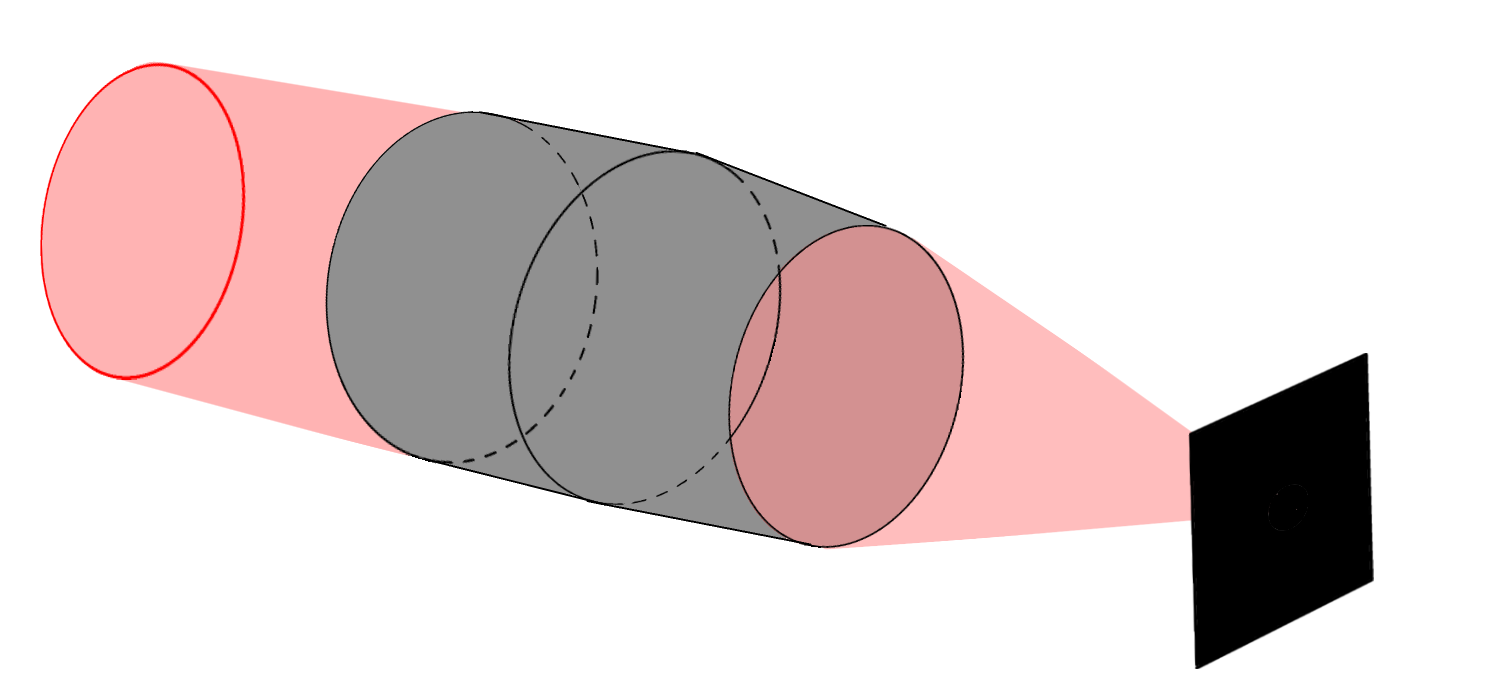
\includegraphics[width=12cm]{solitude_schematic_for_wolter.png}
\caption{Wolterミラー下流端面の孤立条件を用いる方法}
\label{fig:solitude_schematic}
\end{figure}

\subsection{タイコグラフィ法}
\label{chap3_ptychography_introduction}

\subsubsection{タイコグラフィ法の概要}
\ref{chap3_solitude_introduction}節では1枚の画像に対して孤立条件から冗長性を確保して位相回復を行ったが、タイコグラフィ法では光学系に徐々に変化を与えながら、多数の画像を撮影することによって冗長性を確保する。
図\ref{fig:ptychography_schematic}にその概要を示す。

\begin{figure}[!ht]
\centering
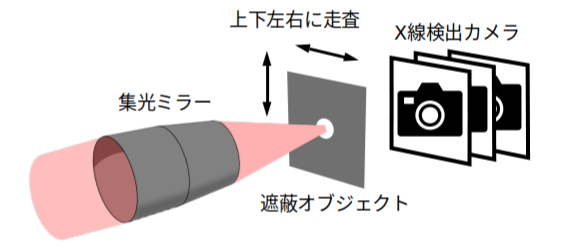
\includegraphics[width=12cm]{ptychography_schematic.png}
\caption{タイコグラフィ法の概要}
\label{fig:ptychography_schematic}
\end{figure}

集光ミラーに設計時に想定された光源からの入射光を入れ、その焦点面にオブジェクトを差し入れる。
このオブジェクトによって変化を受けた波面がさらに下流側に設置されたカメラによって撮影される。
これを、オブジェクトの位置を焦点面内で鉛直および水平方向に走査しながら多数の画像を撮影することで、冗長性を確保するという寸法である。
用いるオブジェクトは大きく分けて2種類ある。
1つはガラスなどの透過性を持つ物体の厚みに適当なパターンを与えた試料をオブジェクトとするものである。
物体の厚みを位置によって変えることで、それに応じて波面の位相の進み量に差が生じる。
試料の作製については、SiO2のエッチングによるパターニングなどが知られている。\cite{Godden2016}
この方法は、タイコグラフィによるミラー評価だけでなく、試料そのものを評価するタイコグラフィ顕微鏡としても利用できる。
もう1つは、ビームを完全に遮蔽できるような金属板に適当な穴を開けて作られるオブジェクトである。
焦点面における波面は完全に遮蔽される部分と完全に透過される部分の2つに分かれ、透過した波面の穴のエッジで回折した光が下流側のカメラに入射する。
これらのオブジェクトを焦点面内で走査し、各位置に対する回折光を

竹尾らは、ピンホール(1つの円形の穴)を開けた板をオブジェクトとして利用し、ピンホールのエッジをなぞるように走査する方法でタイコグラフィを行い、ミラー内面形状の評価に成功している。
ピンホールを用いた方法では、ミラーの内側で反射せず直接通過した光を処理することが位相パターンをつけた試料より容易である。

\subsubsection{PIE}
位相回復法は元来、X線顕微鏡として利用されたため、回復の対象はサンプル(オブジェクト)であった。
その最も簡単なタイコグラフィのアルゴリズムがPIE(Ptychography Iterative Engine)である。
これは、照明関数は既知であるとして与え、オブジェクトのみ回復計算を行うアルゴリズムである。
PIEの疑似コードをAlgorighm\ref{alg:pie}に示す。

\begin{algorithm}                      
\caption{PIE Algorithm}         
\label{alg:pie}                          
\begin{algorithmic}
    \STATE $O_0(\pos) = \mathrm{rand}(0,1) \exp(i \mathrm{rand}(0,1) )$
    \FOR{n = 0 \ldots N-1}
      \FOR{j = 0 \ldots M-1}
        \STATE $\psi(\pos_j) = P(\pos) O_n(\pos_j + \pos)$
        \STATE $\Psi(\rpos) = \mathcal F [\psi(\pos)]$
        \STATE $\Psi'(\rpos) = \sqrt{I_j(\rpos)} \exp\left( i \arg \psi(\pos) \right)$ 
        \STATE $\psi'(\pos) = \mathcal F^{-1} [\Psi'(\rpos)]$
        \STATE $O_{n+1}(\pos + \pos_j)'
          = O_n(\pos + \pos_j) 
          + \frac{P_n^*(\pos)}{|P(\pos)|^2+\varepsilon} \left( \psi_n'(\pos) - \psi_n(\pos) \right)$
      \ENDFOR
    \ENDFOR
\end{algorithmic}
\end{algorithm}

逆空間で拘束を掛け、実空間に戻したあとで、オブジェクトを更新する。
オブジェクトの更新則としてシンプルなのは$\psi(\pos_j) = P(\pos) O_n(\pos_j + \pos)$としたのに対応させて$O_{n+1}(\pos_j + \pos) = \frac{\psi'(\pos_j)}{P(\pos)}$とする方法である。
しかし、これは除算に際して発散が起こる可能性があり、実用上大きな問題を孕んでいる。
これを、式\ref{eqn:object_update_derivation}のように変形する。
\begin{eqnarray}
O_{n+1}(\pos_j + \pos)
  &=& \frac{\psi'(\pos_j)}{P(\pos)} \nonumber \\
  &=& \left( O_n(\pos_j + \pos) - \frac{\psi(\pos_j)}{P(\pos)} \right) + \frac{\psi'(\pos_j)}{P_n(\pos)} \nonumber \\
  &=& O_n(\pos_j + \pos) + \frac{1}{P(\pos)} \left( \psi'(\pos_j) - \psi(\pos_j) \right) \label{eqn:object_update_derivation}
\end{eqnarray}

これを一般化して文字を置き換えると、式\ref{eqn:object_update_simplified}のように書ける。
\begin{equation}
\label{eqn:object_update_simplified}
  O_{n+1}(\pos_j + \pos) = O_n(\pos_j + \pos) + w \Delta\psi(\pos)
\end{equation}
この更新の重み$w$を変えることで、アルゴリズムの改善を図る。
発散を回避するため、重みの分母を実数化して微小な定数$\varepsilon$を足して式\ref{eqn:pie_object_update_weight}のように重みを定めたのがAlgorithm\ref{alg:pie}に示したPIEのアルゴリズムである。
\begin{equation}
  \label{eqn:pie_object_update_weight}
  w = \frac{P^*(\pos)}{\left| P(\pos) \right|^2 + \varepsilon}
\end{equation}

\subsubsection{rPIE}
PIEがオブジェクトのみ回復を行っていたのに対して、照明関数も未知として回復計算を行うのがePIE(exteded PIE)である。
ePIEでは式\ref{eqn:pie_object_update_weight}のように定数で発散を回避するのではなく、式\ref{eqn:epie_object_update_weight}のように絶対値の2乗の最大値を取る。
また、更新係数にハイパーパラメタ$\alpha$を掛けることで収束性を上げることができることが知られている。
\begin{equation}
  \label{eqn:epie_object_update_weight}
  w = \alpha \frac{P_n^*(\pos)}{\max \left| P_n(\pos) \right|^2}
\end{equation}
ePIEでは照明関数も更新しなければいけないが、これはオブジェクトの更新と同様に式\ref{eqn:epie_probe_update}のように行われる。
\begin{equation}
\label{eqn:epie_probe_update}
  P_{n+1}(\pos) 
  = P_n(\pos) 
  + \beta \frac{O_n^*(\pos_j + \pos)}{\max \left| O_n(\pos_j + \pos) \right|^2} \Delta\psi(\pos)
\end{equation}

ePIE(式\ref{eqn:epie_object_update_weight})のように最大値を取る方法に対して、各点での絶対値の2乗とその最大値で重み付き平均を取って分母とするのがrPIE(regularized PIE)である。
更新式は式\ref{eqn:rpie_object_update}および式\ref{eqn:rpie_probe_update}に示す通りである。
rPIEはほとんどePIEの一般化になっている。
\begin{eqnarray}
  O_{n+1}(\pos_j + \pos) &=& O_n(\pos_j + \pos) 
    + \frac{P_n^*(\pos_j + \pos)}
      {\alpha \max \left| P_n(\pos) \right|^2 + (1-\alpha) \left| P_n(\pos) \right|^2}
    \Delta\psi(\pos) \label{eqn:rpie_object_update} \\
  P_{n+1}(\pos) &=& P_n(\pos) 
    + \frac{O_n^*(\pos_j + \pos)}
      {\beta \max \left| O_n(\pos_j + \pos) \right|^2 + (1-\beta) \left| O_n(\pos_j + \pos) \right|^2}
    \Delta\psi(\pos) \label{eqn:rpie_probe_update}
\end{eqnarray}

rPIEのアルゴリズムをAlgorithm\ref{alg:rpie}に示す。

\begin{algorithm}[!ht]
\caption{rPIE Algorithm}         
\label{alg:rpie}                          
\begin{algorithmic}
    \STATE $O_0(\pos) = \mathrm{rand}(0,1) \exp(i \mathrm{rand}(0,1) )$
    \STATE $P_0(\pos) = \mathrm{rand}(0,1) \exp(i \mathrm{rand}(0,1) )$
    \FOR{n = 0 \ldots N-1}
      \FOR{j = 0 \ldots M-1}
        \STATE $\psi(\pos_j) = P_n(\pos) O(\pos_j + \pos)$
        \STATE $\Psi(\rpos) = \mathcal F [\psi(\pos)]$
        \STATE $\Psi'(\rpos) = \sqrt{I_j(\rpos)} \exp\left( i \arg \psi(\pos) \right)$ 
        \STATE $\psi'(\pos) = \mathcal F^{-1} [\Psi'(\rpos)]$
        \STATE $O_{n+1}(\pos_j + \pos) 
          = O_n(\pos_j + \pos) + \frac{P_n^*(\pos_j + \pos)}
          {\alpha \max \left| P_n(\pos) \right|^2 + (1-\alpha) \left| P_n(\pos) \right|^2}
          \Delta\psi(\pos)$
        \STATE $P_{n+1}(\pos)
          = P_n(\pos) + \frac{O_n^*(\pos_j + \pos)}
          {\beta \max \left| O_n(\pos_j + \pos) \right|^2 + (1-\beta) \left| O_n(\pos_j + \pos) \right|^2}
          \Delta\psi(\pos)$
      \ENDFOR
    \ENDFOR
\end{algorithmic}
\end{algorithm}

タイコグラフィ法においても、走査ステップを変えることで回復領域の重なり具合が変化し、この比(オーバーサンプリング比)が収束性を左右する。
ステップが小さいほどオーバーサンプリング比は大きく収束性は高くなるが、その分必要な領域を走査し終えるのに必要な計測時間は増大してしまう。
Bunkらの検討によれば、オーバーサンプリング比が0.6程度が最適であるということが知られている。\cite{Bunk2008}

\subsection{ディテクター走査による冗長性}
\label{chap3_detector_scanninc_introduction}

タイコグラフィ法ではオブジェクトを走査することで冗長性を確保したが、ディテクターを走査することで冗長性を確保する方法も知られている。

\begin{figure}[!ht]
\centering
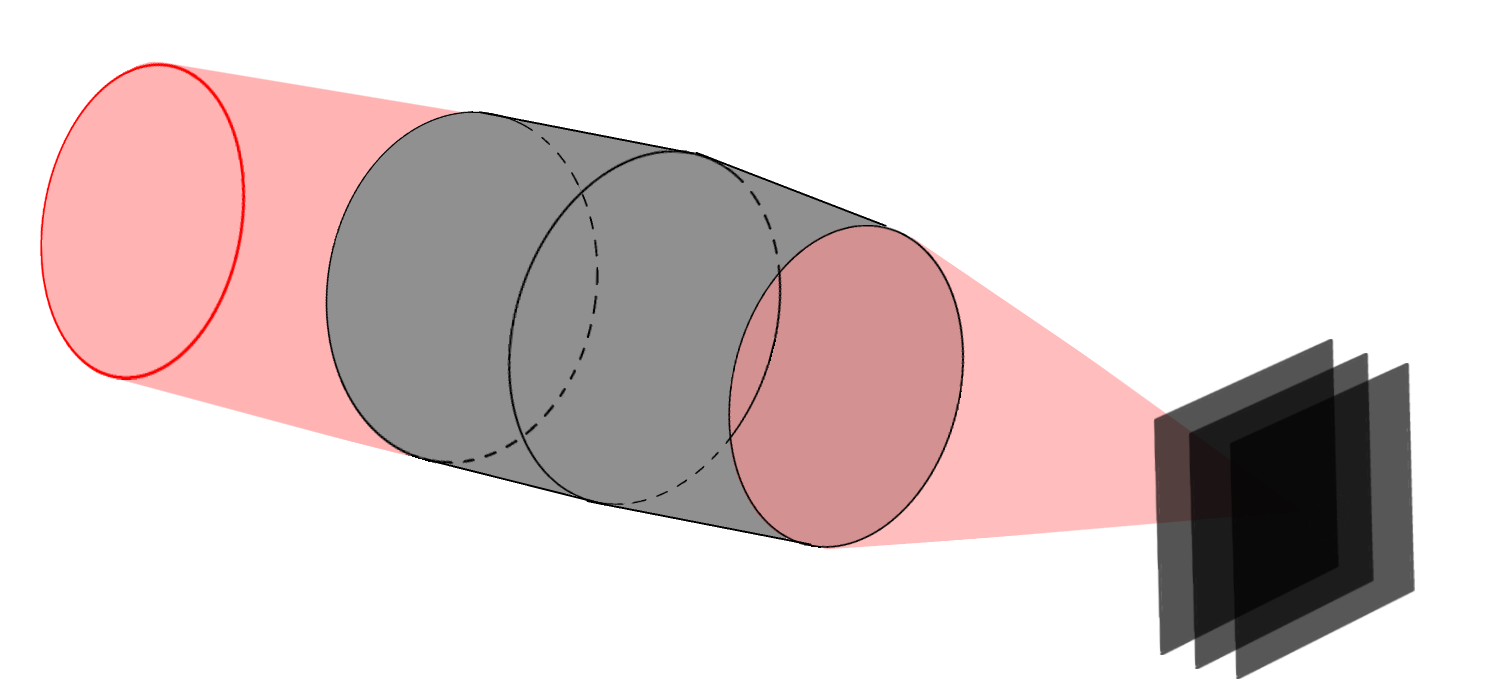
\includegraphics[width=12cm]{detector_scanning_schematic.png}
\caption{ディテクターを走査する方法の概要}
\label{fig:detector_scanning_schematic}
\end{figure}

下流端面から各ディテクター走査位置までの伝播計算は、焦点面までFresnel回折伝播、そこからさらに角スペクトル法でディテクター走査距離ぶんの伝播をするという2段階の構成で行われる。
タイコグラフィ法同様、各面に伝播するごとに強度を計測強度値と置き換える拘束を掛けることを繰り返し位相分布を回復する。

\subsection{下流端開口走査による冗長性}
\label{chap3_transverse_introduction}

オブジェクトを走査する位置を焦点面ではなく集光素子の開口直後とするTransverse Translation法がBradyらによって提案されている。\cite{Brady2009}
これは図\ref{fig:transverse_schematic}に示すように、焦点面を操作するタイコグラフィ法同様にオブジェクトを集光素子の開口で走査し、その回折像を下流側のカメラで撮影するという方法である。

\begin{figure}[!ht]
\centering
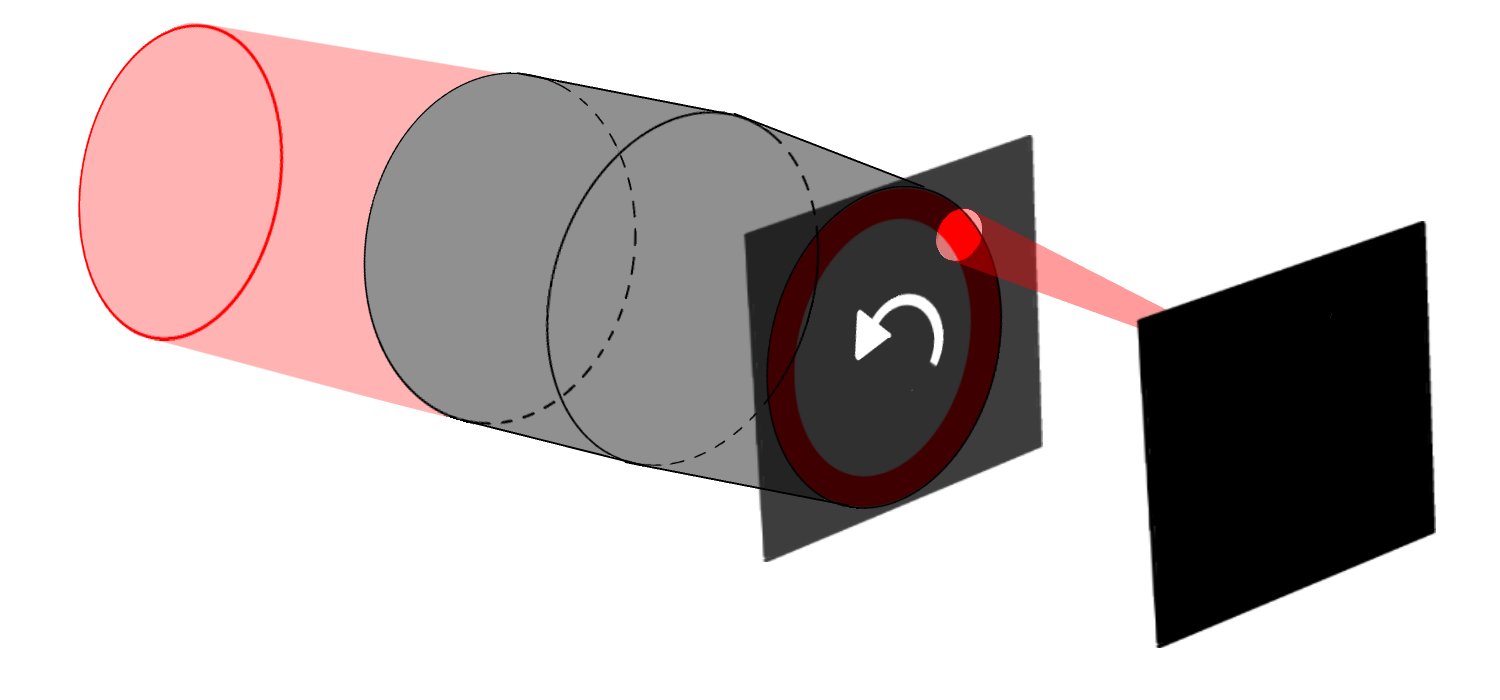
\includegraphics[width=12cm]{transverse_schematic.png}
\caption{Transverse Translation Diversityの概要}
\label{fig:transverse_schematic}
\end{figure}

輪帯はほぼ真円状になっているため、走査には回転ステージが有効である。
計算アルゴリズム自体は基本的にはタイコグラフィ法と同様にすればよく、特にピンホール形状の曲率誤差が問題にならない場合はピンホールは既知の円形状として与え、HIOとPIEを混合したアルゴリズムを用いればよい。

\clearpage
% ================================================== %
% section
% ================================================== %
\newpage

\section{手法の比較・決定}

\subsection{分解能に関する検討}
\label{chap3_comparison_resolution}

計測によって得られる下流端面の空間分解能を比較する上で最も重要なのは、位相回復計算の対象となる2つの平面がどこに設定されているかということである。
この観点で比較すると、上に挙げた4つの手法は孤立条件(\ref{chap3_solitude_introduction}節)、ディテクター走査(\ref{chap3_detector_scanninc_introduction}節)、下流端面走査(\ref{chap3_transverse_introduction})の3つと焦点面走査(\ref{chap3_ptychography_introduction})の2種類に大別される。
前者は下流端面と焦点面(近傍)におかれたCCD面、後者は焦点面に置かれたオブジェクト平面とそれよりさらに下流にあるCCDカメラの受光面が回復計算の対象となる。
\ref{chap3_sampling_theorem}節で述べたサンプリング定理に基づいて考えると、下流端面の空間分解能が高いことは焦点面における回復領域が大きいことに対応する。
前者の方法では、焦点面の回復領域の大きさはCCDカメラの受光面の大きさによって決まる。
\ref{chap3_dynamic_range}節に示したCCDを利用し、CCD全面に渡って回復計算を行うことができたとすれば、下流端面の1画素の一辺は\SI{32.66}{\micro \metre}であり、輪帯を動径方向に11.13ピクセルの分解能で計測できる。
一方で、後者の方法では焦点面の回復領域の大きさは走査面積によって決まり、その走査全体で必要となる撮影回数はCCDカメラの画素サイズによって決まる。
一方で焦点面走査の場合、1枚の画像に対応して回復される領域サイズはビームの焦点強度分布においてメインローブの数倍から10倍程度であり、前者と同じ36.9 mmの領域を回復するためには、10万枚オーダーの撮影が必要になる。
1枚の撮影に数秒程度かかるとすればこれは計測時間が現実的なものではなく、今回のWolterミラー計測には適さない。

\subsection{ダイナミックレンジに関する検討}
\label{chap3_comparison_dynamic_range}

続いて、焦点面にCCDカメラを配置する残り3つの手法について、ダイナミックレンジに関する検討を行う。
図\ref{fig:single_pinhole_mask}のように下流端面に$\Phi 4.5$ mmのピンホールを入れた場合、およびオブジェクトを何も挿入せず焦点面に光を集めた場合について、その集光面強度分布を図\ref{fig:comparison_focus_pinhole_existence}に示す。
また、水平方向プロファイルを強度ピークで規格化して比較したものが図\ref{fig:transverse_dynamic_range_speriority}である。
全面照明の場合は集光点付近に強度分布が集中しているのに対して、ピンホールを挿入すると広範囲に渡って分布していることが分かる。
このことから、ピンホールを挿入する方が、ダイナミックレンジに対応して有効領域が狭まるということが起きにくく、より安定した回復計算の収束が期待できる。

\begin{figure}[!ht]
\centering
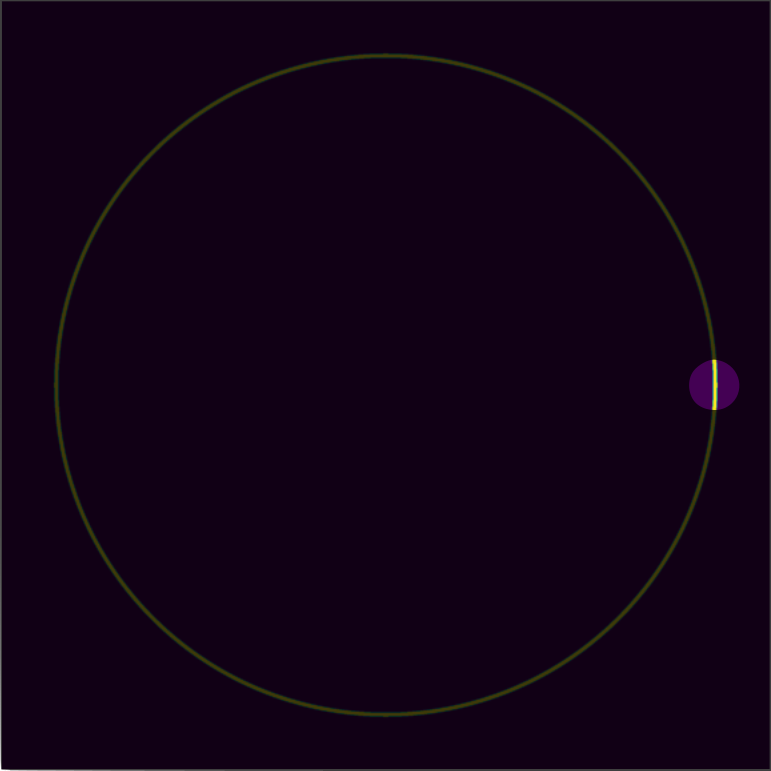
\includegraphics[width=6cm]{single_pinhole_masked_ring.png}
\caption{下流端面でのピンホールの模式図}
\label{fig:single_pinhole_mask}
\end{figure}


\begin{figure}[!ht]
\centering

\subfloat[オブジェクトがない場合]{
    
\includegraphics[width=6cm]{full_field_focus.png}
    \label{fig:full_field_focus}
}
\subfloat[$\Phi 4.5$ mmのピンホールを挿入した場合]{
    \centering
    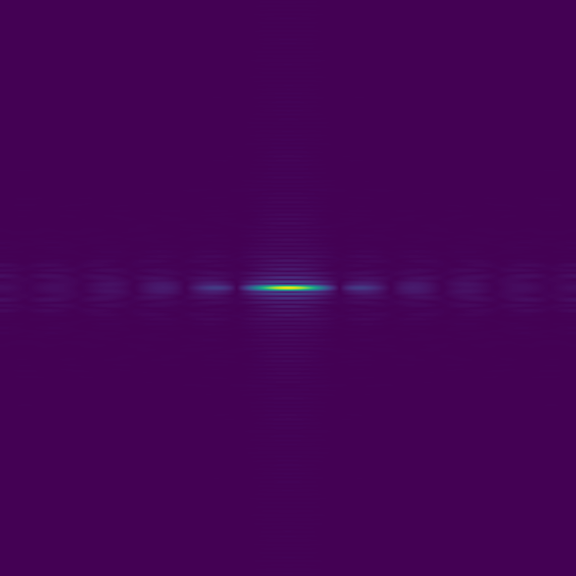
\includegraphics[width=6cm]{single_pinhole_focus.png}
    \label{fig:single_pinhole_focus}
}

\caption[]{ピンホールの有無による焦点面強度分布の比較}
\label{fig:comparison_focus_pinhole_existence}
\end{figure}

\begin{figure}[!ht]
\centering
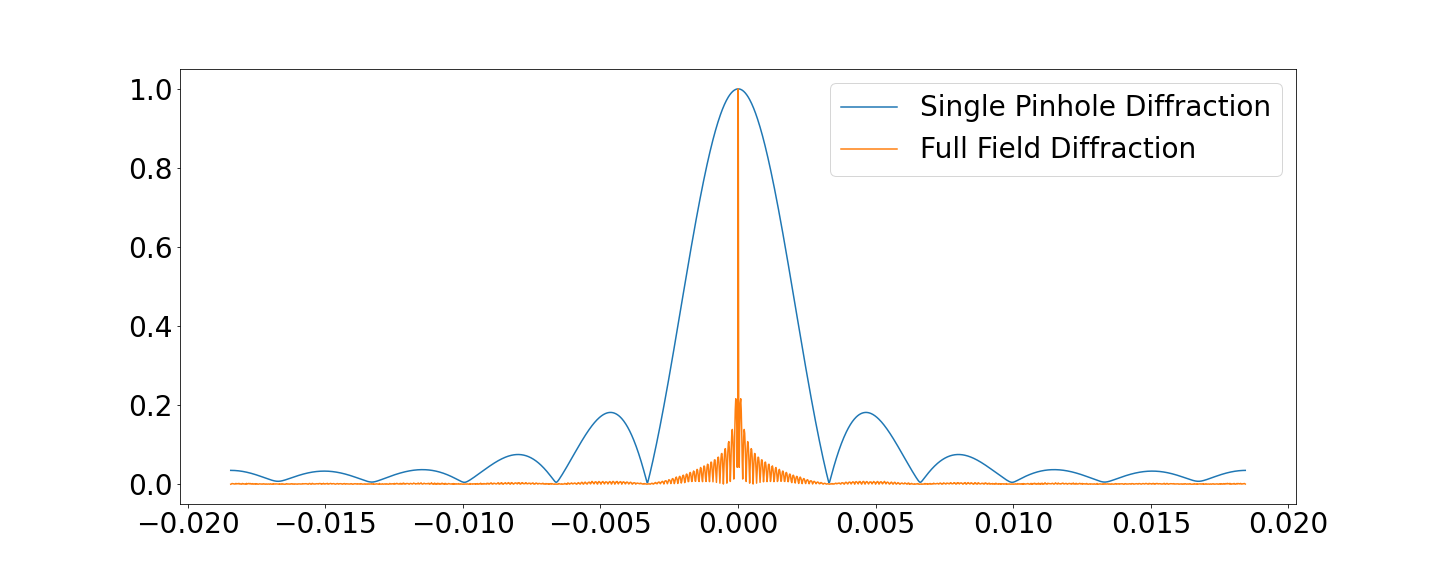
\includegraphics[width=14cm]{pinhole_dynamic_range_superiority.png}
\caption{ピンホールの有無による焦点面強度プロファイルの比較}
\label{fig:transverse_dynamic_range_superiority}
\end{figure}

\subsection{手法の選択}
\label{chap3_decision_of_method}
空間分解能に関する議論、およびダイナミックレンジに関する議論から、\ref{chap3_transverse_introduction}節の下流端に挿入したオブジェクトを走査する方法が最も安定して高い空間分解能での測定を実現すると結論づけ、これを測定手法として採用する。

\clearpage
% ================================================== %
% section
% ================================================== %
\newpage

\section{手法の提案}
\label{chap3_transverse_arrangement}

下流端開口面を走査する方法について、その構成を検討する。
\ref{chap3_comparison_dynamic_range}節で図\ref{fig:single_pinhole_focus}に示したように、ピンホールを挿入した際の理想的な輪帯に対して焦点面の強度分布は対称になっている。
つまり、輪帯上の半周ずれた点にピンホールを置いた場合と焦点面強度分布が変わらないため、焦点面における拘束が波面を解に近づけるとは限らない。
実際、\ref{fig:single_pinhole_mask}の構成において位相回復計算シミュレーションを行ったが、波面は正しく回復されなかった。
Bradyらの計測においては、焦点面よりも下流側にCCDカメラを配置することで非対称化を図っている。\cite{Brady2009}
例として、500 mm下流側における強度分布を角スペクトル法で計算すると図\ref{fig:single_pinhole_defocus}のようにデフォーカスし、対称性が崩れる。

\begin{figure}[!ht]
\centering
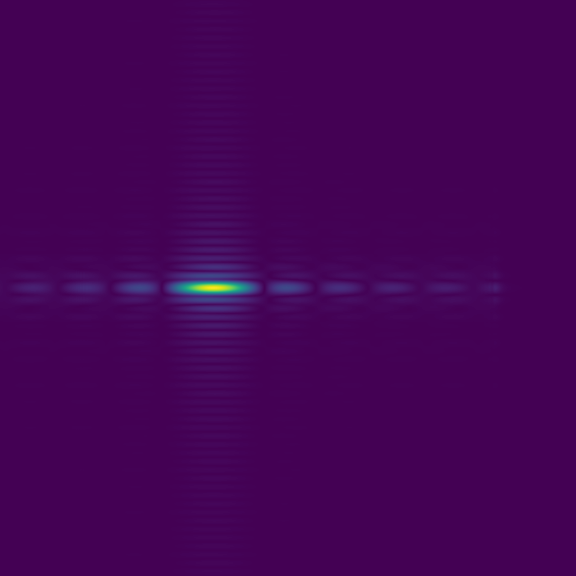
\includegraphics[width=6cm]{single_pinhole_defocus.png}
\caption{焦点面から500 mm下流側での強度分布}
\label{fig:single_pinhole_defocus}
\end{figure}

この方法の欠点として、焦点位置を調整したあとに移動を行うために位置決め精度が必要であること、回復計算ごとに線状畳み込みが必要な角スペクトル法での計算が必要となり計算時間が大きくなってしまうことが挙げられる。

\subsection{不等間隔複数ピンホールによる非対称化}
デフォーカスを用いない方法として、ピンホールを複数配置することで非対称性をもたせるという手法を提案する。
ピンホール2つでは、ピンホールが2つの場合と状況が変わらず、位相を回復することができない。
ピンホール2つを対称に配置し、さらにそこから角度をずらした位置にピンホールを配置することにより、非対称性を生み出すことができる。
図\ref{fig:three_pinhole_mask}はその一例として、対称な位置に2つとそこから45度ずれた位置にピンホールを挿入した場合について示した。

\begin{figure}[!ht]
\centering
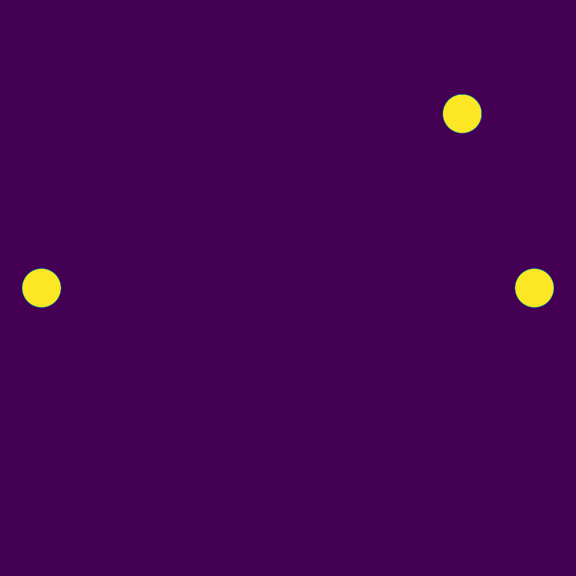
\includegraphics[width=6cm]{three_pinhole_mask.png}
\caption{不等間隔ピンホールの例}
\label{fig:three_pinhole_mask}
\end{figure}

このようにピンホールを配置すると、焦点面における強度分布は図\ref{fig:three_pinhole_focus}のようになる。

\begin{figure}[!ht]
\centering

\includegraphics[width=6cm]{three_pinhole_focus.png}
\caption{不等間隔ピンホールの例}
\label{fig:three_pinhole_focus}
\end{figure}


\clearpage
% ================================================== %
% section
% ================================================== %
\newpage

\section{提案手法に関するシミュレーション}
\label{chap3_transverse_simulation}

本節では、まず位相回復計算およびシミュレーションに必要な光学波動場の伝播計算、および位相回復結果の解析に必要となる位相接続について述べた上で、提案手法についてシミュレーションを行い、その結果を示す。

\subsection{Wolterミラーにおける光学波動場の伝播}
\label{chap3_wolter_diffraction_apporoximation}
シミュレーションおよび位相回復計算を行うにあたり、測定対象のWolterミラーの光学系において適用するべき波動場伝播の近似公式について検討する。
光学波動場の伝播に関しての詳細は付録において解説する。
まず、1章\ref{chap1_wolter_arrangement}節で示したパラメータについて、Fresnel回折近似の成立条件が成り立っているかどうかを確認する。
Fresnel回折近似が成り立つための条件は、近似で切り捨てる微小項が1 radより十分小さいときであり、これは式\ref{eqn:fresnel_approximation_condition}で表される。
ただし$z$は伝搬距離、$\lambda$は波長、$(x, y), (\xi, \eta)$は実空間および逆空間の座標を表す。

\begin{equation}
\label{eqn:fresnel_approximation_condition}
    \frac{\pi}{4\lambda} \max \left\{ (x-\xi)^2 + (y-\eta)^2 \right\}^2 / z^3 \ll 1
\end{equation}

焦点面を3章\ref{chap3_dynamic_range}節に示したCCDカメラのサイズとして取りこれを計算すると、(左辺)の値は1.645 radとなった。
これは十分小さいとは言えず、Fresnel回折近似を満たしているとは言えない。
しかし、Fresnel回折近似を満たしていない場合でも、計算を進めていく上でそれがほとんど影響を及ぼさない場合がある。
位相回復計算においては数万回の伝搬計算を行うため、1回のコストは最小限であることが好ましい。
そこで、厳密計算であるRayleigh-Sommerfeld回折積分とFresnel回折積分近似の集光面強度分布を比較し、実用上の問題が存在するかどうかを検討する。
まず、表\ref{tb:check_approximation_validity_1}に示すような適当な分割で回折積分を実行し、集光波面分布におけるメインピークのFWHMを調べる。

\begin{table}[!ht]
\begin{center}
  \begin{tabular}{|c|c|} \hline
    項目 & 値 \\ \hline
    波長 & 632.8 nm \\
    画素数 & $2048 \times 2048$ \\
    焦点面ピクセルサイズ & \SI{5.0}{\micro \metre} \\ \hline
  \end{tabular}
  \caption{Fresnel回折近似適用可能性の検討1}
  \label{tb:check_approximation_validity_1}
\end{center}
\end{table}

計算の結果、プロファイルは図\ref{fig:fwhm_approximation}のようになった。

\begin{figure}[ht]
\centering
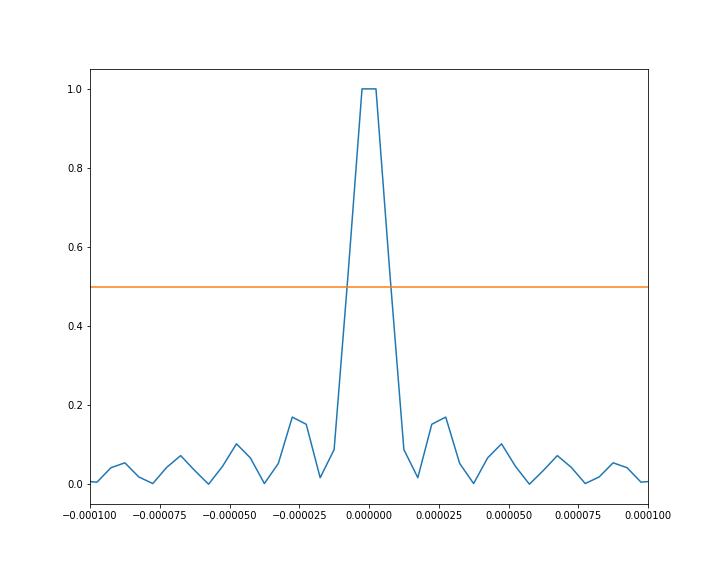
\includegraphics[width=8cm]{../../chap2/figure/fwhm_approximation.png}
\caption{回折積分計算による簡易的な計算で得られた焦点面強度プロファイル}
\label{fig:fwhm_approximation}
\end{figure}

ここから計算されるFWHMは4ピクセル分の\SI{20}{\micro \metre}であった。
これを踏まえ、メインピークを十分な分割数で観察できるよう焦点面ピクセルサイズが\SI{1}{\micro \metre}になるような表\ref{tb:check_approximation_validity_2}のパラメータで回折積分およびFresnel回折近似を用いた場合の集光面強度プロファイルを計算し、比較を行う。

\begin{table}[!ht]
\begin{center}
  \begin{tabular}{|c|c|} \hline
    項目 & 値 \\ \hline
    波長 & 632.8 nm \\
    画素数 & $4096 \times 4096$ \\
    焦点面ピクセルサイズ & \SI{1.0}{\micro \metre} \\ \hline
  \end{tabular}
  \caption{Fresnel回折近似適用可能性の検討2}
  \label{tb:check_approximation_validity_2}
\end{center}
\end{table}

計算の結果、プロファイルは図\ref{fig:diffraction_comparison}のようになった。
また、2つのプロファイルの差分を取って回折積分の最大値で規格化したグラフが図\ref{fig:diffraction_comparison_normalized_diff}である。

\begin{figure}[!ht]
\centering

\subfloat[プロファイルプロット]{
    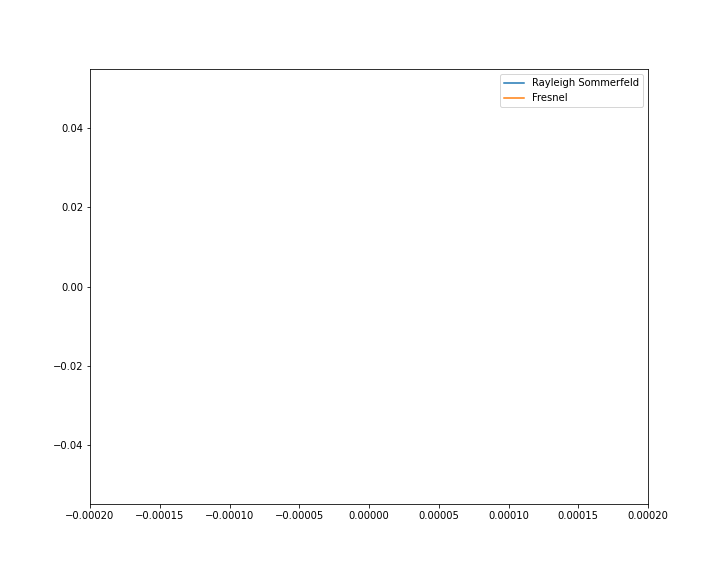
\includegraphics[width=6cm]{../../chap2/figure/diffraction_comparison_profile.png}
    \label{fig:diffraction_comparison_profile}
}
\subfloat[規格化されたプロファイル誤差]{
    \centering
    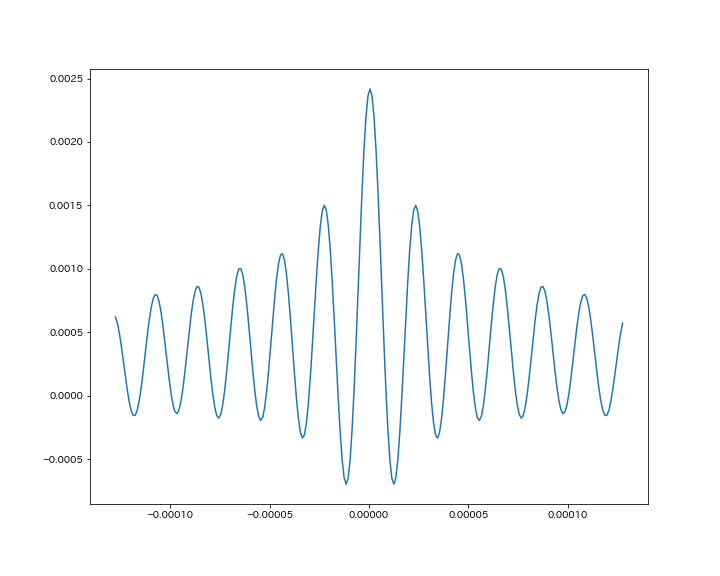
\includegraphics[width=6cm]{../../chap2/figure/diffraction_comparison_normalized_diff.png}
    \label{fig:diffraction_comparison_normalized_diff}
}

\caption[]{Rayleigh-Sommerfeld回折積分とFresnel回折積分のプロファイル比較}
\label{fig:diffraction_comparison}
\end{figure}

差分の絶対値の最大値は0.00242程度となった。
これは十分小さく、実際の計測で生じうるノイズと同程度以下であるため、シミュレーションでの検討および位相回復計算を行う上で致命的な問題をもたらさない。
ゆえに、以降の伝搬計算はFresnel回折近似を用いて行う。

\subsection{位相接続(位相アンラッピング)}
$\sin$関数などの周期関数は、逆関数の値域が周期以下の大きさしか持たないため、完全にもとの入力を戻すことはできない。
複素波動場の位相分布についても同様である。
$\exp(i\phi)$は周期$2\pi$の関数であり、逆関数は$\arg\{\exp(i\phi)\}=\phi \mod{2\pi}$と位相の$\mod{2\pi}$での剰余を返す。
故に、位相分布が本来なめらかな関数として与えられたとしても、それが$2\pi$を超えるような範囲に渡って分布する際には必ずどこかで不連続に位相が飛んでしまう。
例えば、$y = f(x) = 10x + 20x^2 \quad (x \in [0, 1])$に対して$z = \arg\{\exp(iy)\}$を取ると、図\ref{fig:wrapped_graph_example}のようになる。

\begin{figure}[ht]
\centering
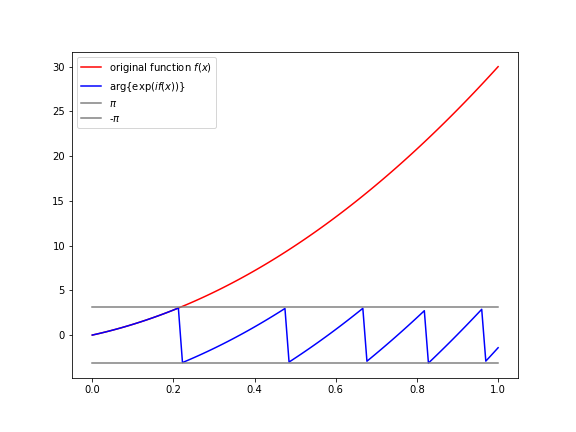
\includegraphics[width=10cm]{before_unwrap.png}
\caption{arg関数によって不連続になったグラフの例}
\label{fig:wrapped_graph_example}
\end{figure}

これに対して、離散化された領域において1ピクセルで$2\pi$以上のジャンプはないものと仮定して順番に接続を行うことで、なめらかな位相分布を取り戻すことができる。
これを位相接続あるいは位相アンラップといい、1次元の離散列$y[n] = f(x[n])$および$z[n]=\arg\{\exp(iy[n])\}$に対して最もシンプルなアルゴリズムはAlgorithm \ref{alg:unwrap_1d}のようになる。
連続した位置を走査していき、1つ前のピクセルと$\pi$以上の位相差が生じたらそれ以降の点全てに$2\pi$を足し引きし、位相を接続する。

\begin{algorithm}                      
\caption{1次元アンラップの例}         
\label{alg:unwrap_1d}                          
\begin{algorithmic}
    \FOR{$n = 1 \ldots N-1$}
        \STATE $\delta = \begin{cases}
                -2 \pi & (z[n] + \pi < z[n]) \\
                0 & (z[n] - \pi \leq z[n] \leq z[n] + \pi) \\
                2 \pi & (z[n] < z[n] - \pi)
            \end{cases}$
        \FOR{$k = n \ldots N-1$}
            \STATE $z[k] \leftarrow z[k] + \delta$
        \ENDFOR
    \ENDFOR
\end{algorithmic}
\end{algorithm}

2次元のリング状の領域に対しても同様にできる。
接続するべき2次元位相分布内においてその順序を決めれば、1次元の場合と同じアルゴリズムで接続を行うことができる。
本研究では、まず図\ref{fig:unwrap_transform}のように$x-y$座標から$\theta-r$の極座標分布に変換する。
その上で図\ref{fig:unwrap_path}のように$r$方向の中央部分を$\theta$方向に走査したのちにその各点から各$\theta$について動系方向に走査するといった順序でAlgorithm \ref{alg:unwrap_1d}を適用し、最後に$x-y$座標系に戻す。
ミラー波面計測においては、経験的に十分な空間分解能があれば$2\pi$以上のジャンプはないと考えてよいとされており、本研究でも同様にその仮定をおいて測定を行う。

\begin{figure}[!ht]
\centering
\subfloat[$x-y$座標における位相分布]{
    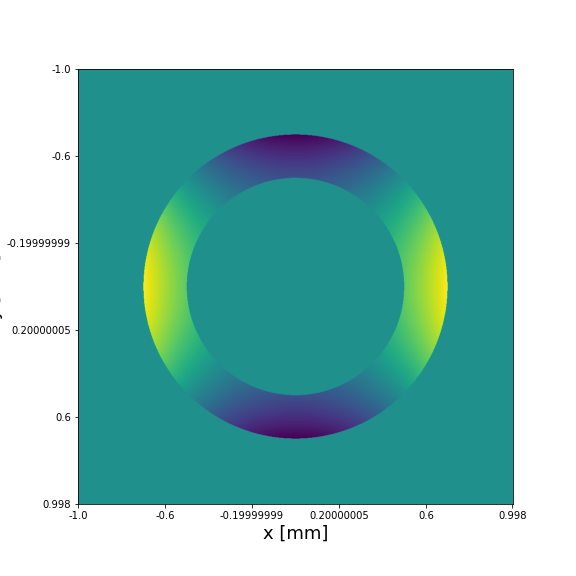
\includegraphics[width=6cm]{unwrap_xy.png}
    \label{fig:unwrap_xy}
}
\subfloat[極座標における位相分布]{
    \centering
    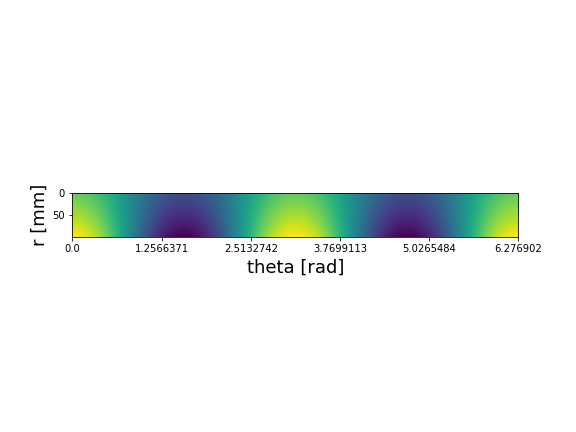
\includegraphics[width=6cm]{unwrap_polar.png}
    \label{fig:unwrap_polar}
}
\caption[]{位相分布の座標変換}
\label{fig:unwrap_transform}
\end{figure}

\begin{figure}[!ht]
\centering
\subfloat[$x-y$座標に対応させた走査経路]{
    \centering
    \includegraphics[width=6cm]{unwrap_path.png}
    \label{fig:unwrap_path_xy}
}
\subfloat[極座標での走査経路]{
    \centering
    \includegraphics[width=6cm]{unwrap_path_polar.png}
    \label{fig:unwrap_path_polar}
}
\caption[]{位相分布の座標変換}
\label{fig:unwrap_path}
\end{figure}

\subsection{位相回復シミュレーションの結果}
\label{chap3_transverse_simulation_result}

現実の測定において現れる非点収差が存在する場合についてシミュレーション上の測定を行い、位相回復計算を行った。
図\ref{fig:sim_transverse}に入力波面および回復された波面を、また図\ref{fig:sim_profile_comparison}に輪帯幅の半分に当たる位置での周方向位相分布を比較したグラフを示す。
入力した位相分布に対して、回復計算が正しく収束し、波面が回復されていることが確認できる。

\begin{figure}[!ht]
\centering
\subfloat[入力した波面]{
    \centering
    \includegraphics[width=6cm]{sim_answer.png}
    \label{fig:sim_answer}
}
\subfloat[回復された波面]{
    \centering
    \includegraphics[width=6cm]{sim_reconstructed.png}
    \label{fig:sim_reconstructed}
}
\caption[]{位相回復シミュレーションの結果}
\label{fig:sim_transverse}
\end{figure}

\begin{figure}[ht]
\centering
\includegraphics[width=10cm]{sim_profile_comparison.png}
\caption{回復波面と入力波面の輪帯中央でのプロファイル比較}
\label{fig:sim_profile_comparison}
\end{figure}

\clearpage
% ================================================== %
% section
% ================================================== %
\newpage


\section{結論}
\label{chap3_conclusion}

位相回復法の中で空間分解能およびダイナミックレンジの観点から優れていると考えられる下流端面走査法について、非対称化の方法として不等間隔に穴を配置したオブジェクトの利用を提案した。
また、シミュレーションの結果から位相回復計算が正しく行われることを確認し、手法としての正当性を検証した。


%%%%%%%%%%%%%%%%%%%%%%%%%%%%%%%%%%%%%%%%%%%%%%%%%%%%%%%%%%%%%%%%%%%%%%%%%%%%%
%%% Local Variables:
%%% mode: katex
%%% TeX-master: "../thesis"
%%% End:

%\chapter{レンズによる提案手法の検討}
\thispagestyle{empty}
\label{chap4}
\graphicspath{{chap4/figure/}}
\minitoc

\newpage
%%%%%%%%%%%%%%%%%%%%%%%%%%%%%%%%%%%%%%%%%%%%%%%%%%%%%%%%%%%%%%%%%%%%%%%%%%%%%


% ================================================== %
% section
% ================================================== %
\section{諸言}
\label{chap4_introduction}

本章では5章のミラー測定実験に先立って、ほぼ理想的と言える集光光学系に対して3章で提案された手法による計測実験を行い、その正当性を検証する。
具体的な方法としては、平行光に対して輪帯状の開口を入れ、さらにレンズによって集光することで、輪帯状の集光球面波を作ることができ、擬似的にミラー下流端面を再現する。
再現された擬似的な輪帯に対して位相回復法が適用出来れば、細い輪帯形状の波面回復法に対して提案手法が有効的であることがいえ、また本研究の測定対象である天文用Wolterミラーに対してもその適用可能性が大きいということが言える。
また、1層のWolterミラーの波面計測のための手法検討に加えて、Nested Wolterミラーにも同手法が適用可能であるかどうかを検討するための実験を行う。
現時点では入手性の観点から実際のNested Wolterミラーを計測することは難しいが、Nested Wolterミラーの集光波面を模倣した輪帯に対して位相回復法が機能すれば、十分に応用可能であることの根拠を与える。
\ref{chap4_experiment_setup}節では、実験の構成およびそれに含まれる各光学素子のパラメータ等について示す。


\clearpage
% ================================================== %
% section
% ================================================== %
\newpage

\section{実験の構成および設計パラメータ}
\label{chap4_experiment_setup}

\ref{chap4_introduction}節で述べたとおり、本章ではほぼ理想的な輪帯上の集光波面を擬似的に生成し、これに対して波面計測を行う。
輪帯上の集光波面は、図\ref{fig:psuedo_focusing_ring_model}に示すように輪帯アパーチャ及び集光レンズによって生成される。

\begin{figure}[!ht]
\centering
\includegraphics[width=13cm]{psuedo_focusing_ring.png}
\caption{疑似的な輪帯状集光ビームの生成}
\label{fig:psuedo_focusing_ring_model}
\end{figure}

疑似輪帯を用いた計測実験は、本来の測定対象であるWolterミラーと同様の光学的パラメータで構成されるべきだが、入手性の問題からここではレンズとして口径は異なるがNAがWolterミラーのそれとほぼ等しいレンズを用いる。
用いたレンズのパラメータは表\ref{tb:focusing_lens_params}に示す通りである。

\begin{table}[h]
\begin{center}
  \begin{tabular}{|c|c|} \hline
    パラメータ & 値 \\ \hline
    直径 & 30.0 mm  \\
    焦点距離 & 1000.000 mm \\
    設計波長 & 541.6 nm \\ \hline
  \end{tabular}
  \caption{レンズの設計パラメータ}
  \label{tb:focusing_lens_params}
\end{center}
\end{table}

これに合わせて、輪帯開口および位相回復に用いるピンホールを図\ref{fig:lens_pinhole_ring_aperture}の用に設計した。

\begin{figure}[!ht]
\centering

\subfloat[輪帯アパーチャ]{
    \centering
    \includegraphics[width=6cm]{ring_aperture.png}
    \label{fig:lens_ring_aperture}
}
\subfloat[ピンホール]{
    \centering
    \includegraphics[width=6cm]{pinhole_arrangement.png}
    \label{fig:lens_pinhole_arrangement}
}
\caption[]{設計図面}
\label{fig:lens_pinhole_ring_aperture}
\end{figure}

\clearpage
% ================================================== %
% section
% ================================================== %
\newpage


\section{疎条件を利用した位相回復の結果}
回復計算に用いたパラメータは以下の通りである。

回復計算が収束しなかった。


\clearpage
% ================================================== %
% section
% ================================================== %
\newpage

\section{下流端走査によるタイコグラフィの結果}


\subsection{半周のみ走査した場合のタイコグラフィの結果}

\subsection{繰り返し計測の結果}

像が回復できることが確認されたため、さらに10回の繰り返し計測を行い、繰り返し再現性およびその波面計測の精度を確認する。


\clearpage
% ================================================== %
% section
% ================================================== %
\newpage

\section{Nested Wolterミラーに対する下流端走査型位相回復法の検証}

1層の場合と同様に、輪帯状の集光波面が同心円状に2つ存在するような状況を擬似的に作り出し、これを計測する。
アパーチャとピンホールの設計を図\ref{fig:lens_nested_pinhole_ring_aperture}に示す。

\begin{figure}[!ht]
\centering

\subfloat[輪帯アパーチャ]{
    \centering
    \includegraphics[width=6cm]{nested_ring_aperture.png}
    \label{fig:lens_nested_ring_aperture}
}
\subfloat[ピンホール]{
    \centering
    \includegraphics[width=6cm]{nested_pinhole_arrangement.png}
    \label{fig:lens_nested_pinhole_arrangement}
}
\caption[]{疑似Nested Wolter計測用の設計図面}
\label{fig:lens_nested_pinhole_ring_aperture}
\end{figure}

\subsection{結果}

回復された波面の強度分布を図\ref{fig:result_nested_restored_abs}に示す。

\begin{figure}[!ht]
\centering
\includegraphics[width=6cm]{result_nested/restored_abs.png}
\caption{疑似的な輪帯状集光ビームの生成}
\label{fig:result_nested_restroed_abs}
\end{figure}



\clearpage
% ================================================== %
% section
% ================================================== %
\newpage


\section{結論}
\label{chap4_conclusion}


%%%%%%%%%%%%%%%%%%%%%%%%%%%%%%%%%%%%%%%%%%%%%%%%%%%%%%%%%%%%%%%%%%%%%%%%%%%%%
%%% Local Variables:
%%% mode: katex
%%% TeX-master: "../thesis"
%%% End:

\chapter{ミラー計測実験}
\thispagestyle{empty}
\label{chap5}
\graphicspath{{chap5/figure/}}
\minitoc

\newpage
%%%%%%%%%%%%%%%%%%%%%%%%%%%%%%%%%%%%%%%%%%%%%%%%%%%%%%%%%%%%%%%%%%%%%%%%%%%%%


% ================================================== %
% section
% ================================================== %
\section{諸言}
\label{chap5_introduction}

本章では、実際に天文用Wolterミラーを\ref{chap3}章の提案手法による計測実験を行い、その解析を行う。
測定対象となるミラーは、東京大学の三村グループによって2021年1月に作製された天文用Wolterミラーであり、これらの設計パラメータは1章\ref{chap1_wolter_arrangement}に示した通りである。
この3枚のミラーそれぞれについて位相回復計算を行った結果、およびその繰り返し計測精度と回転角度を変えた場合の整合性について述べる。

\clearpage
% ================================================== %
% section
% ================================================== %
\newpage

\section{実験の構成}

実験装置の概要を図\ref{fig:mirror_experiment_schematic}に示す。
まず、レーザーからビームを出力し、これをNDフィルタによって減衰させ、強度を調整する。
次に、レンズを2つ使ってビームを拡大し平行化する。
これを測定対象のWolterミラーに入射し、さらにタイコグラフィのための回転ピンホールを通過させる。
最後に、一番下流にあるCCDカメラで強度分布を撮影する。

\begin{figure}[!ht]
\centering
\includegraphics[width=13cm]{mirror_experiment_schematic.png}
\caption{ミラー測定実験系 模式図}
\label{fig:mirror_experiment_schematic}
\end{figure}

これらの光学素子のパラメータを表\ref{tb:mirror_experiment_params}に示す。
なお、NDフィルタは実験によって適宜ピークがダイナミックレンジに収まるように設定されるため、そのパラメータ等を記述しない。

\begin{table}[h]
\begin{center}
  \begin{tabular}{|c|c|} \hline
    パラメータ & 値 \\ \hline
    ビーム波長 & 632.8 nm  \\
    ビームサイズ($\text{TEM}_{00} 1/e^2$点 +3\%) & 0.63 mm  \\
    ビーム発散角度($\text{TEM}_{00}$ +3\%) & 1.3 mrad  \\
    拡大用レンズ焦点距離 & 8.0 mm  \\
    平行化用レンズ焦点距離 & 800.0 mm  \\
    拡大倍率 & 100 倍 \\
    レンズ設計波長 & 541.6 nm \\ \hline
  \end{tabular}
  \caption{Wolterミラー計測実験装置における各素子のパラメータ}
  \label{tb:mirror_experiment_params}
\end{center}
\end{table}

これらを構成した実験装置のCAD図を以下に示す。図\ref{fig:mirror_experiment_asm_cad_side}が横から見た図、図\ref{fig:mirror_experiment_asm_cad_isometric}が俯瞰して見た図である。

\begin{figure}[!ht]
\centering
\includegraphics[width=14cm]{asm_total_side.png}
\caption{ミラー測定実験系 側面図}
\label{fig:mirror_experiment_asm_cad_side}
\end{figure}

\begin{figure}[!ht]
\centering
\includegraphics[width=10cm]{asm_total_isometric.png}
\caption{ミラー測定実験系 俯瞰図}
\label{fig:mirror_experiment_asm_cad_isometric}
\end{figure}


\subsection{ミラーの把持}
回転体ミラーの測定実験系を構成する上で、ミラーの把持は一つの問題となる。
板型ミラーの場合であれば、反射面以外の平面部を挟むようにして把持することができる。
一方で円筒型の薄いミラーの場合そのような部分はなく、できるだけ小さな応力で、かつ設置位置に決まった位置に収まるように把持しなければならない。
そこで、仙波らの方法にならい、Bessel点で触れるように下から把持する機構を採用する。\cite{Senba2010}
Bessel点は均等荷重を受ける2点支持された梁の重力によるたわみ量が最小となるような点であり、梁の全長$L$に対して、梁の両端から内側に向かって約$0.2203L$(あるいは中心から$\pm 0.2797 L$)の位置として計算される。
ミラーは光軸上の位置によって半径が異なり厳密には均等荷重ではないが、斜入射が小さくほぼ真円筒とみなせるため、近似的な範囲ではこれで十分であると考えた。
測定対象のミラー全長220 mmに対してBessel点は中心から約$\pm$61.53 mmであり、これを採用した把持機構は図\ref{fig:mirror_holder_jig}のようになった。
ミラーと治具の接触点は赤点で示す通りである。

\begin{figure}[!ht]
\centering
\includegraphics[width=10cm]{mirror_holder_jig.png}
\caption{ミラー把持部の設計図}
\label{fig:mirror_holder_jig}
\end{figure}

また、ミラーを置き直した際に設置位置の繰り返し再現性が高い方が、アラインメントに関して有利である。
光軸方向の距離を合わせるため、ミラー上流端においてミラーの厚み1mmに対してちょうどその半分の位置に当たるような治具を配置し、これに対して押し付けるようにミラーを設置した。
実際に組み立てられた装置は図\ref{fig:photo_mirror_experiment_mirror_and_pinhole}のようになった。

\begin{figure}[!ht]
\centering
\includegraphics[width=5cm]{photo_mirror_pinhole.png}
\caption{ミラー測定実験系 写真}
\label{fig:photo_mirror_experiment_mirror_and_pinhole}
\end{figure}


\subsection{ピンホールの設計}

ピンホールの設計は図\ref{fig:mirror_pinhole_arrangement}に示す通りである。
断りとして、以下の設計が2つの誤謬を孕んでいることを述べておく。
1つは、ピンホール中心が移動する円の直径はちょうど計測する輪帯状波面のちょうど半分の直径とするのが自然だが、そのような直径を持つ円に対して1つのピンホールが対応する角度を先に決めて、その角度を持つ扇形の弦が直径となるように円を定めている。
もう1つは、シミュレーション上で回復ができると判断した半径2.25 mmの円に対して、直径2.25 mmとしてしまったことである。
これによって、上の計算にはもはや意味を失っている。
ただ、測定対象の輪帯がピンホール通過領域に収まれば問題はなく、直径の決め方は些細な問題である。

\begin{figure}[!ht]
\centering

\subfloat[ピンホールの設計]{
    \includegraphics[width=7cm]{pinhole_arrangement.png}
    \label{fig:mirror_pinhole_arrangement}
}
\subfloat[回転半径の決め方]{
    \centering
    \includegraphics[width=6cm]{pinhole_arrangement_policy.png}
    \label{fig:mirror_pinhole_arrangement_policy}
}
\caption[]{ピンホールの設計}
\label{fig:pinhole_arrangement_pictures}
\end{figure}


\clearpage
% ================================================== %
% section
% ================================================== %
\newpage

\section{計測波面以外の通過光の処理方法に関する検討}
測定対象となっている天文用Wolterミラーは、X線集光用に設計・作製されたものであり、可視光を入射した際にどのような集光波面が生じるかは未検討である。
\ref{chap4}章での提案手法の検討は、あくまで波面計測の対象である輪帯のみが存在する場合について行われたが、実際にミラーを計測する実験においては測定対象以外の光も通過してCCDカメラの方向に進行する。
円形の平行光を入射した際にミラーより下流に通過する光は、図\ref{fig:mirror_beam_path_types}に示す通り3種類存在する。
1つは計測対象の2回反射光、1つは放物面には当たらず双曲面で1回だけ反射された光、1つは直接通過光である。

\begin{figure}[!ht]
\centering
\includegraphics[width=10cm]{reflection_beam_types.png}
\caption{ミラーに入射した光の進路}
\label{fig:mirror_beam_path_types}
\end{figure}

直接通過光は、ピンホールの金属板によって遮蔽されており、またピンホールを通過してもCCDカメラの撮影領域から10 mm以上外れているためこれは計測強度値に影響を及ぼさない。
双曲面による一回反射光は、焦点面において直径約30 mmとなるため、CCDカメラに入射してしまう。
これを取り除く方法は2種類考えられる。
1つは、撮影される強度分布において1回反射光を含まない領域を切り出し、これを回復に用いる方法、もう1つは集光点より上流に存在する1回反射光の集まる位置でこれを遮蔽するという方法である。
前者では切り出しを行ったとしてもその回折光は入射してしまうほか、焦点面サイズを狭めることになるため下流端面の空間分解能が低下してしまう。
後者では集光ビームを遮ることなく遮蔽することはほとんど不可能である上、遮蔽板のエッジで回折した光はまた焦点面の強度分布に影響を及ぼしてしまう。
いずれも大きな問題を抱えているが、本実験では構成が簡単な前者を選択することとする。


\clearpage
% ================================================== %
% section
% ================================================== %
\newpage

\section{撮影条件およびデータの処理}

\subsection{撮影条件}
撮影時の条件を表

\begin{table}[!ht]
\begin{center}
  \begin{tabular}{|c|c|} \hline
    パラメータ & 値 \\ \hline
    CCDカメラ設定温度 & \SI{20}{\degreeCelsius}  \\ \hline
  \end{tabular}
  \caption{Wolterミラー計測実験の条件}
  \label{tb:mirror_experiment_params}
\end{center}
\end{table}

\subsection{ダークフレームの計測}
\label{chap5_darkflame_measurement}

入射ビームを遮断した場合においても、CCDカメラの検出する強度は0とはならない。
実験室を完全に暗転できないこと、CCDカメラに壊れている素子が存在していること、熱によるノイズの発生などの要因によって、測定対象の各ピクセルの強度値にはシステムエラーが生じる。
以下ではこれに対して適切な対策を施すため、計15枚のダークフレームを取得し、その代表的統計値を計算する。
15枚のダークフレームから統計的に得られる情報として、画像内での強度のばらつきおよび撮影ごとのばらつきがある。
まず、平均ダークフレーム中における統計情報を表\ref{tb:darkflame_average_data}および図\ref{fig:pinhole_arrangement_pictures}に示す。
ただし、平均ダークフレームは15枚の単純平均によって計算した。
ヒストグラムは、全体が中央値付近に偏って分布しているため、領域を絞って表示している。

\begin{table}[!ht]
\begin{center}
  \begin{tabular}{|c|c|} \hline
    パラメータ & 値 \\ \hline
    最大値 & 62444.36 \\
    最小値 & 1063.60 \\
    平均値 & 1113.45 \\
    中央値 & 1113.07 \\
    標準偏差 & 60.8071 \\ \hline
  \end{tabular}
  \caption{15枚のダークフレームの平均の統計情報}
  \label{tb:darkflame_average_data}
\end{center}
\end{table}

\begin{figure}[!ht]
\centering

\subfloat[1次元化した平均ダークフレーム強度分布]{
    \includegraphics[width=7cm]{darkflame_average_ravel.png}
    \label{fig:darkflame_average_ravel}
}
\subfloat[ダークフレームのヒストグラム]{
    \centering
    \includegraphics[width=7cm]{darkflame_average_histogram.png}
    \label{fig:darkflame_average_histogram}
}

\caption[]{平均ダークフレームにおける統計情報}
\label{fig:darkflame_average_stat}
\end{figure}

続いて、ダークフレームの撮影ごとの変化について目を向け、各ピクセルごとに求められるダークフレームに関しての統計情報を示す。

\begin{table}[!ht]
\begin{center}
  \begin{tabular}{|c|c|} \hline
    パラメータ & 値 \\ \hline
    最大値 & 3040.99 \\
    最小値 & 4.10 \\
    平均値 & 15.46 \\
    中央値 & 15.33 \\
    標準偏差 & 4.11 \\ \hline
  \end{tabular}
  \caption{ダークフレームの標準偏差の統計情報}
  \label{tb:darkflame_deviation_data}
\end{center}
\end{table}

\begin{figure}[!ht]
\centering

\subfloat[1次元化したダークフレーム標準偏差の強度分布]{
    \includegraphics[width=7cm]{darkflame_deviation_ravel.png}
    \label{fig:darkflame_deviation_ravel}
}
\subfloat[ダークフレーム標準偏差のヒストグラム]{
    \centering
    \includegraphics[width=7cm]{darkflame_deviation_histogram.png}
    \label{fig:darkflame_deviation_histogram}
}

\caption[]{ダークフレーム標準偏差における統計情報}
\label{fig:darkflame_deviation_stat}
\end{figure}

平均ダークフレームに関して、全体として1000程度のオフセットがあり、これは実験室内の機器の光が漏れてCCDカメラに入射しているものと考えられる。
またごく少数(20ピクセル程度)ではあるが、10000を超えるような値を取っているピクセルがあり、そのようなピクセルの標準偏差はいずれも1\%以下程度であるためこれは素子が不能になっているものと考えられる。
また15枚のダークフレーム間での標準偏差に関して、この平均値は十分に小さく撮影ごとの変化は大きくないと言える。

\subsection{ダークフレームの除去}
\ref{chap5_darkflame_measurement}節の計測により、ダークフレームの撮影ごとの変化はかなり小さいこと、また実験室内に存在する外乱光の影響で全体に1000程度の強度が乗ることが分かった。
外乱光の除去のため、計測開始の直前に計8枚のダークフレームを取得し、単純加算平均の結果を計測データから差し引いた。

\clearpage

% ================================================== %
% section
% ================================================== %
\newpage

\section{下流端走査タイコグラフィの結果}
\label{chap5_mirror_transverse_result}

\subsection{回復結果}

\begin{figure}[!ht]
\centering
\subfloat[回復された位相分布]{
    \includegraphics[width=7cm]{reconstructed_phase_before_unwrap.png}
    \label{fig:reconstructed_phase_before_unwrap}
}
\subfloat[位相アンラップ後の位相分布]{
    \centering
    \includegraphics[width=7cm]{reconstructed_phase_unwrapped.png}
    \label{fig:reconstructed_phase_unwrapped}
}
\caption[]{回復された位相分布の位相アンラップ}
\label{fig:reconstructed_phase_unwrapping}
\end{figure}


\begin{figure}[!ht]
\centering
\subfloat[回復された位相分布(極座標)]{
    \includegraphics[width=7cm]{reconstructed_phase_before_unwrap_polar.png}
    \label{fig:reconstructed_phase_before_unwrap_polar}
}
\subfloat[位相アンラップ後の位相分布(極座標)]{
    \centering
    \includegraphics[width=7cm]{reconstructed_phase_unwrapped_polar.png}
    \label{fig:reconstructed_phase_unwrapped_polar}
}
\caption[]{回復された位相分布の位相アンラップ(極座標)}
\label{fig:reconstructed_phase_unwrapping_polar}
\end{figure}

輪帯幅のちょうど半分に当たる部分について回転角度方向にプロファイルを取ると、非点収差にあたる$\sin(\theta)$の成分が現れた。
これを$A \sin(\theta + \theta_0)$の形で最小自乗フィッテイングして重ねたものが図\ref{fig:astigmatism_fitted}である。
また、その差分を図\ref{fig:astigmatism_canceled}に示す。

ここで、真円度測定器RoncorderEC1550によって測定された周方向誤差プロファイルを図\ref{fig:roundness_error}に示す。
図\ref{fig:roundness_error_each}は上流側(放物面側)からの光軸方向距離$z$に応じてその周方向誤差を計測したプロファイルであり、図\ref{fig:roundness_error_average}はその単純平均である。

\begin{figure}[!ht]
\centering
\subfloat[光軸方向の各位置での周方向誤差プロファイル]{
    \includegraphics[width=7cm]{roundness_error_each.png}
    \label{fig:roundness_error_each}
}
\subfloat[平均化された周方向誤差プロファイル]{
    \centering
    \includegraphics[width=7cm]{roundness_error_average.png}
    \label{fig:roundness_error_average}
}
\caption[]{真円度測定器での周方向誤差プロファイル測定結果}
\label{fig:roundness_error}
\end{figure}

回復された位相の周方向分布においてフィッティングされた非点収差成分は、その振幅が7.68 rad ($1.22\lambda$)であった。
これを周方向誤差量に換算すると\SI{101.5}{\micro \metre}程度になり、これがミラーによるものであるとすると真円度測定結果と大きく矛盾するため、非点収差がミラーに起因するものであるかどうかを確認する。
焦点面における強度分布を撮影すると、図\ref{fig:astigmatism_focus_before_rotation}のようであり、確かに集光点が円形ではなく十字の広がりを持っており、非点収差が存在することが確認できる。
続いて、ミラーを45度程度回転し、同様に焦点面における強度分布を撮影したものが図\ref{fig:astigmatism_focus_after_rotation}である。
ミラーに起因する非点収差であればミラーの回転に伴って集光点のパターンが回転するはずだが、ほとんど変わらない分布を示している。
これにより、位相回復結果から算出された非点収差はミラーより上流側の入射ビームの生成において生じたものであると結論付けることができる。

また、図\ref{fig:reconstructed_focus}に回復された波面から計算される焦点面の強度分布を示す。
直接撮影された焦点面強度分布とよく一致しており、位相回復計算に大きな誤謬が無いことが確認できた。


\begin{figure}[!ht]
\centering
\subfloat[輪帯中央における位相分布とsinフィッティング]{
    \includegraphics[width=7cm]{astigmatism_fitted.png}
    \label{fig:astigmatism_fitted}
}
\subfloat[非点収差成分を差し引いた位相分布]{
    \centering
    \includegraphics[width=7cm]{astigmatism_canceled.png}
    \label{fig:astigmatism_canceled}
}
\caption[]{回復された位相分布の位相アンラップ(極座標)}
\label{fig:astigmatism_analysis}
\end{figure}


\begin{figure}[!ht]
\centering
\subfloat[回転前の焦点面強度分布]{
    \includegraphics[width=7cm]{before_rotation.png}
    \label{fig:astigmatism_focus_before_rotation}
}
\subfloat[回転後の焦点面強度分布]{
    \centering
    \includegraphics[width=7cm]{after_rotation.png}
    \label{fig:astigmatism_focus_after_rotation}
}
\caption[]{回転前後の焦点面強度分布}
\label{fig:darkflame_deviation_stat}
\end{figure}


\begin{figure}[!ht]
\centering
\includegraphics[width=8cm]{reconstructed_focus.png}
\caption{回復された波面から計算される焦点面強度分布}
\label{fig:reconstructed_focus}
\end{figure}


% ================================================== %
% section
% ================================================== %
\section{結論}
\label{chap5_conclusion}

波面計測法として機能させることは出来なかったが、入射ビームの非点収差が位相回復計算によって算出され、実際に入射ビームによる影響であるという結論が得られた。
位相回復法自体に大きな誤りが無いことも確認されたことから、入射ビームを調整し、再度計測を行うことによりミラーの形状誤差を正しく反映した位相分布を計測可能であると考えられる。


%%%%%%%%%%%%%%%%%%%%%%%%%%%%%%%%%%%%%%%%%%%%%%%%%%%%%%%%%%%%%%%%%%%%%%%%%%%%%

%%% Local Variables:
%%% mode: katex
%%% TeX-master: "../thesis"
%%% End:

\chapter{結論}
\thispagestyle{empty}
\label{chap6}
\graphicspath{{chap6/figure/}}
\minitoc

\newpage
%%%%%%%%%%%%%%%%%%%%%%%%%%%%%%%%%%%%%%%%%%%%%%%%%%%%%%%%%%%%%%%%%%%%%%%%%%%%%


% ================================================== %
% section
% ================================================== %
\section{提案手法の適用可能性}
\label{chap6_conclusion}




\clearpage


% ================================================== %
% section
% ================================================== %
\newpage

\section{今後の展望}
\label{chap6_futureworks}


\clearpage
\newpage


%%%%%%%%%%%%%%%%%%%%%%%%%%%%%%%%%%%%%%%%%%%%%%%%%%%%%%%%%%%%%%%%%%%%%%%%%%%%%
%%% Local Variables:
%%% mode: katex
%%% TeX-master: "../thesis"
%%% End:


% ++++++++++++++++++++++++++++++++++++++++++++++++++++++++++++++++ %
%   Appendix
% ++++++++++++++++++++++++++++++++++++++++++++++++++++++++++++++++ %
%\appendix
%\chapter{付録}
\lhead[付録]{}
\label{appendix}
\graphicspath{{figure/}}
\minitoc

\newpage
\section{光学波動場の伝播}
\subsection{Kirhihoff-Helmholtz方程式}

\subsection{Rayleigh-Sommerfeldの回折積分公式}

\subsection{Rayleigh-Sommerfeldの高速計算}

\subsection{Fresnel回折積分}

\subsection{Fraunhofer回折積分}

\subsection{角スペクトル法}


%%%%%%%%%%%%%%%%%%%%%%%%%%%%%%%%%%%%%%%%%%%%%%%%%%%%%%%%%%%%%%%%%%%%%%%%%%%%%%%
%%% Local Variables:
%%% mode: katex
%%% TeX-master: "../thesis"
%%% End:

%\cleardoublepage

% ++++++++++++++++++++++++++++++++++++++++++++++++++++++++++++++++ %
%   References
% ++++++++++++++++++++++++++++++++++++++++++++++++++++++++++++++++ %
%\chapter*{参考文献}
%\addcontentsline{toc}{chapter}{参考文献}
%\lhead[参考文献]{}
%\renewcommand{\refname}{引用文献}
\thispagestyle{empty}

\bibliography{references}
\bibliographystyle{junsrt}

\newpage

% ++++++++++++++++++++++++++++++++++++++++++++++++++++++++++++++++ %
%  Acknowledgements
% ++++++++++++++++++++++++++++++++++++++++++++++++++++++++++++++++ %
\chapter*{謝辞}

卒業論文を執筆するにあたり、1年間指導して頂いた三村秀和准教授に深い感謝の意を示します。
COVID-19の影響もあり例年とは異なる状況の中で、様々なことに配慮しながら私の進行状況を見守り、導いて下さいました。
充実した研究生活を送ることができたのは、ひとえに先生が環境づくりに努めて下さっているからです。
本当にありがとうございました。
国枝正典教授には、合同研究会での鋭い指摘を頂き、また実験に際して追加工が必要な際には重要な助言をして下さいました。
深く御礼申し上げます。
木村先生には、他愛も無いものから技術的に重要なことまで様々な質問に対して適切な応対をして頂き、作業が滞った際には有効的な助言を頂きました。
オフラインでの研究活動が遅れた私が楽しく研究室に馴染むことが出来たのは先生のおかげです。
ありがとうございました。
技術専門職員の齋さんには、実験装置に必要な部品の追加工を快く引き受けて頂き、おかげでスムーズに計測実験を行うことが出来ました。
深く感謝致します。

上級生として指導に当たって下さった竹尾さん、島村さんはどんなに些細な質問でも優しく親身になって答えてくださり、右も左も分からなかった私に本当に多くのことを教えて下さいました。
山口さんには、ミラーの設計やX線天文学について多くのことを教わりました。
その他大勢の先輩方も、新しく入ってきた私を優しく迎え入れ、充実した研究室生活をサポートして下さいました。

一筋縄では行かず、苦労の多い一年ではありましたが、多くの方々に支えられ、無事に卒業研究を終えることが出来ました。
本当に感謝の念が耐えません。

最後になりますが、これまで私を支え育ててくれた両親、また私を励ましてくれたすべての友人に感謝し、卒業論文の結びと致します。

\markboth{謝辞}{}
\label{thankyou}

\lhead[謝辞]{}
\thispagestyle{empty}

\newpage

\begin{flushright}
2021年1月20日 渡辺 貴史
\end{flushright}

%%%%%%%%%%%%%%%%%%%%%%%%%%%%%%%%%%%%%%%%%%%%%%%%%%%%%%%%%%%%%%%%%%%%%%%%%%%%%%%

%%%%%%%%%%%%%%%%%%%%%%%%%%%%%%%%%%%%%%%%%%%%%%%%%%%%%%%%%%%%%%%%%%%%%%%%%%%%%%%
%%% Local Variables:
%%% mode: katex
%%% TeX-master: "../thesis"
%%% End:
% \addcontentsline{toc}{chapter}{謝辞} %   /* add acknowledgement to the table of contents */

% End of Document
\end{document}